%%%%% Document Setup %%%%%%%%

\documentclass[10pt, twocolumn]{revtex4}    % Font size (10,11 or 12pt) and column number (one or two).

\usepackage{times}                          % Times New Roman font type

\usepackage[a4paper, left=1.85cm, right=1.85cm,
 top=1.85cm, bottom=1.85cm]{geometry}       % Defines paper size and margin length

%\usepackage[font=small,
%labelfont=bf,justification=justified,format=plain]{caption}                      % Defines caption font size as 9pt and caption title bolded


\usepackage{graphics,graphicx,epsfig,ulem}	% Makes sure all graphics works
\usepackage{amsmath} 						% Adds mathematical features for equations

\graphicspath{{Figs/}}

\usepackage{etoolbox}                       % Customise date to preferred format
\makeatletter
\patchcmd{\frontmatter@RRAP@format}{(}{}{}{}
\patchcmd{\frontmatter@RRAP@format}{)}{}{}{}
\renewcommand\Dated@name{}
\makeatother

\usepackage{fancyhdr}
\usepackage{booktabs}
\usepackage{tabularx}
\usepackage{tabulary}
\usepackage{siunitx}

\pagestyle{fancy}                           % Insert header
\renewcommand{\headrulewidth}{0pt}
\lhead{A. Baldacchino}                          % Your name
\rhead{Determining the Position of Patroclus for the \textit{Lucy} Mission Rendezvous} 
% Your report title               


\usepackage{url}
\def\UrlBreaks{\do\/\do-}
\usepackage[hidelinks]{hyperref}
\usepackage[hyphenbreaks]{breakurl}
\usepackage{float}


\def\bibsection{\section*{References}}        % Position refernce section correctly

%\setlength{\belowcaptionskip}{-10pt}
%\setlength{\intextsep}{5pt}
%\setlength{\textfloatsep}{5pt}

\usepackage{hhline}
\usepackage{array}
\usepackage{booktabs}
\usepackage{multirow}
\renewcommand\tabularxcolumn[1]{m{#1}}
\newcolumntype{Y}{>{\centering\arraybackslash}X}
\newcolumntype{Z}{>{\centering\arraybackslash\hsize=.6\hsize}X}
\newcolumntype{A}{>{\centering\arraybackslash\hsize=.4\hsize}X}
%\newcolumntype{M}[1]{>{\centering\arraybackslash}m{#1}}
%\newcolumntype{C}{>{\centering\arraybackslash} m{6cm} }
\usepackage{gensymb}
%\captionsetup[figure]{justification=justified,singlelinecheck=off}


\newcommand{\scite}[1]{\textsuperscript{\cite{#1}}}
\newcommand{\Lucy}{\textit{Lucy }}


%%%%% Document %%%%%
\begin{document}                     

\title{Determining the Position of Patroclus for the \textit{Lucy} Mission Rendezvous} 
\date{Submitted: 25th April 2018}
\author{A. Baldacchino, Lab Partner: L. Thomson}
\affiliation{\normalfont L3 Astrolab, Epiphany Term}

\begin{abstract}              

The aim of this investigation was to study the Trojan asteroid Patroclus to determine its position for the 2033 flyby of the \textit{Lucy} mission. Determining positions accurately is important to space agencies so they can perform orbital manoeuvres successfully and minimise the fuel required for their missions. Observations of a sample of 10 asteroids were taken over the course of 7 weeks, recording their Right-Ascensions and Declinations. This data was used in conjunction with archival data to increase the accuracy of the determined orbital parameters. The mean fractional uncertainty in the orbital parameters for Patroclus was improved from $8.1 \times 10^{-4}$ to $3.5 \times 10^{-7}$ with the inclusion of archival data. This increase in accuracy reduced the confidence volume of the error ellipsoid for Patroclus' position by a factor of ${\sim}10^{11}$. This result is significant as high accuracy is required when performing orbital manoeuvres in order to achieve a flyby with a low relative distance between the spacecraft and the target object. 

\end{abstract}

\maketitle
\thispagestyle{plain} % produces page number for front page

\section{Introduction} 

Jupiter's Trojan asteroids are made up of two groups, the Greek camp and the Trojan camp, which are positioned at Jupiter's L4 and L5 Lagrange points respectively. At the time of writing, there are ${\sim}7{,}000$ asteroids currently classified as Trojans with an asymetry in their distributions: the L4 point has ${\sim}4{,}600$ asteroids and the L5 point has ${\sim}2{,}400$.\textsuperscript{\cite{ListJupiterTrojans}} Studying these asteroids is important to understanding the evolution of the early solar system; they can act as physical indicators of the conditions of the nebula in which they formed.

There is discussion in the literature as to how Jupiter's Trojans formed. Theories have varied and included being captured early in Jupiter's growth,\scite{FlemingoriginTrojanasteroids2000} by collisions,\scite{ShoemakerTrojanasteroidsPopulations1989} and due to the effects of gas drag.\scite{KortenkampCaptureTrojanAsteroids2001} Emery et al, (2015) discuss gas drag and capture during Jupiter's formation in more detail.\textsuperscript{\cite{EmeryComplexHistoryTrojan2015}} However, none  of these methods can account for the broad ${\sim}40\degree$ range in orbital inclinations of their orbits that are observed and has warranted further theories to be explored.

Morbidelli et al, (2005) performed simulations exploring how the asteroids could have been captured immediately after Jupiter and Saturn crossed the $2{:}1$ mean motion resonance (MMR).\textsuperscript{\cite{MorbidelliChaoticcaptureJupiter2005a}} Their results match the orbital distribution of the observed Trojan asteroids and can account for the large distributions in inclinations.
 
Nesvorn\'y et al, (2013) build on the theory proposed by Morbidelli et al, (2005) developing their `Jumping Jupiter' model. Instead of a smooth migration over the $2{:}1$ MMR, it was instead thought that it `jumped' from $2$ to $2.3$ when Jupiter and Saturn scattered off Uranus, Neptune or another body of similar mass.\scite{NesvornyCaptureTrojansJumping2013} This model also matches the orbital distributions of the observed Trojans and they propose that it could account for the asymmetry in the L4-L5 distributions with an ice giant passing near the the L5 point and depleting it of its bodies.

Due to the uncertain nature of the Trojan asteroids, and the lack of direct measurement by man-made satellites NASA approved the \textit{Lucy} missionarger which is planned to launch in October 2021. The aim of this mission is to investigate six of Jupiter's Trojans with its final flyby being of Patroclus in Jupiter's Trojan camp in March 2033. 

Patroclus was selected as a worthwhile object to explore as it is one of the largest in its class of objects and is also in a binary system with its moon Menoetius, which is highly uncommon.\scite{BuieSIZESHAPESTELLAR2015} Observations of Patroclus can be used to calculate the orbital parameters of this binary system and can derrive low densities suggesting that Patroclus could contain a large amount of water ice. This leads to the conclusion it was likely formed in the outer parts of the solar system.\scite{Marchislowdensity8gcm32006}\scite{YangSpectroscopicSearchWater2006} The \textit{Lucy} mission will perform observations using infrared spectrometers and high-resolution imaging devices that will resolve these outstanding questions. 

For this mission to be able to proceed, the orbits of the bodies it plans to visit must be well defined. This allows an efficient flight plan to be constructed that minimises the amount of fuel required, and hence the total cost of the mission. It is also important that the tolerances in the orbital parameters measured are well known. As there is an error in the predicted position for asteroids at any given time, the mission is required to include some reserve fuel so that the spacecraft would still be able to reach its targets at the limits of their known tolerances.

The orbits of bodies can be determined through observations. If the body is observed on at least three different occasions and its Right Ascension (RA) and Declination (Dec) are measured, its orbital parameters can be determined. A body's orbital parameters completely define its Keplerian orbit and traditionally those six elements are: eccentricity ($e$), semi-major axis ($a$), inclination ($i$), longitude of the ascending node ($\Omega$), argument of periapsis ($\omega$) and true anomaly ($\nu$). The parameters are represented in Fig. \ref{fig: orbital params}.

\begin{figure}[h!]
\centering
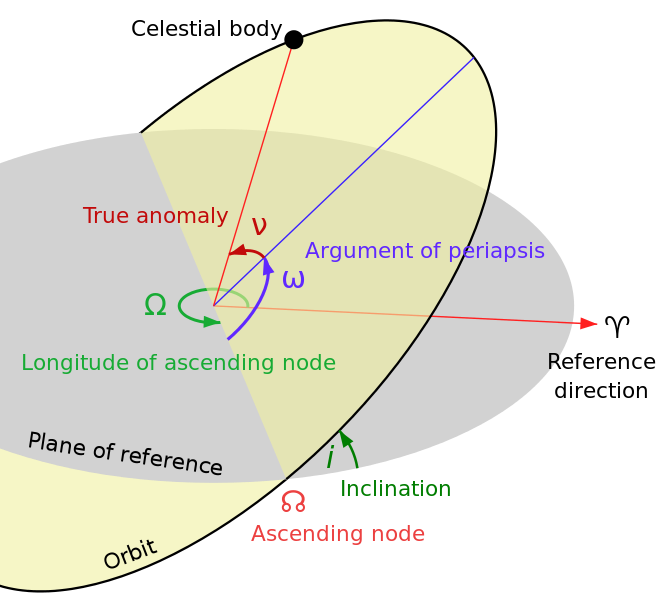
\includegraphics[width=0.5\textwidth]{Orbit1.png}
\caption{A diagram of the orbital parameters typically used to define the orbit of a celestial body in the heliocentric frame. The longitude of ascending node ($\Omega$), true anomaly ($\nu$), argument of periapsis ($\omega$) and inclination ($i$) are shown.\scite{FileOrbit1svg}}
\label{fig: orbital params}
\end{figure}

\begin{figure}[h!]
\centering
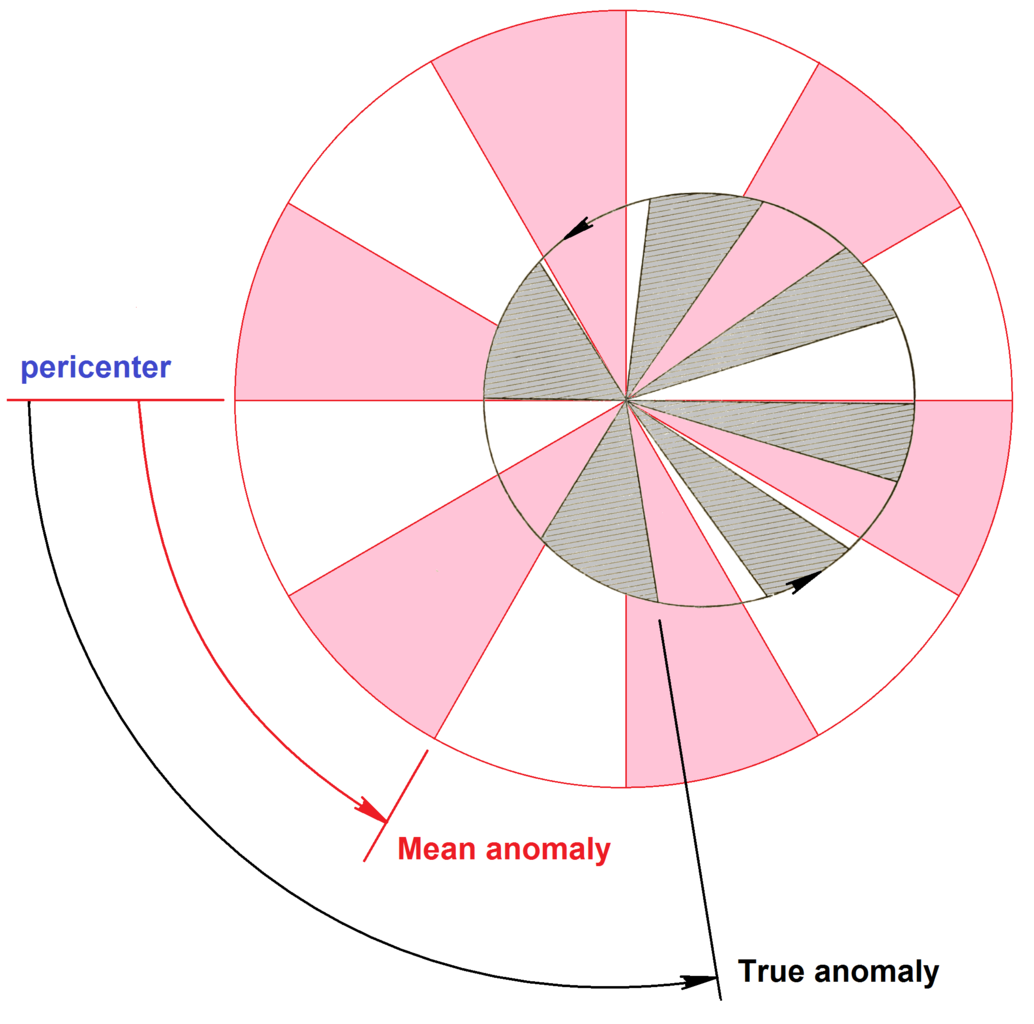
\includegraphics[width=0.5\textwidth]{Mean_anomaly_diagram.png}
\caption{A diagram comparing the mean anomaly and true anomaly orbital parameters in the plane of the orbit. The true anomaly corresponds to the angle on the ellipse at which the body is at. The mean anomaly corresponds to the position on the circle at which the body would be located, mean anomaly increases linearly with time.\scite{Meananomalydiagram2015}}
\label{fig: mean-true anom}
\end{figure}

In this investigation the mean anomaly, $M$, is used in place of the true anomaly, $\nu$. The true anomaly is defined as the angle between the periapsis-focus vector to the object-focus vector in the orbital plane. The mean anomaly is defined as the angle in the orbital plane between the periapsis-focus vector and the imaginary object-focus vector where the object is projected onto a circular orbit around the same body with the same orbital period where an equal area is swept out in a specific time. The main difference between these parameters is that $M$ increases linearly in time whereas $\nu$ does not necessarily behave in the same way if the objects orbit is elliptical. The difference in these parameters is demonstrated in Fig. \ref{fig: mean-true anom}.

As minor body's are easily influenced by the more massive bodies in the solar system, it is not correct to assume that their orbits are Keplerian. When a minor bodies orbital parameters are calculated, they should also be quoted with an epoch of osculation, generally, the date and time these parameters were calculated. This is so that the Keplerian orbit can be perturbed to take account of gravity from other bodies in the solar system, radiation pressure, atmospheric drag and other effects. This results in the body's orbital path not being identical for each rotation which is in contradiction to the classical Keplerian orbit.

In this investigation we calculate the orbits of several Trojan asteroids, including the asteroid Patroclus, using clear band observations of the bodies. We find the accuracy to which we can measure these orbits in order to determine the tolerances on the position of the asteroid Patroclus when \textit{Lucy} plans to rendezvous with it in March~2033.

\section{Method}

Initially, a sample of asteroids was selected that would be visible to us using our available equipment and time frame, our sample being further restricted to the Trojan camp of Jovian asteroids as this was the only group that was visible to us. The asteroids that we chose were: 1974 FV1, Anchises, Ilioneus, Memnon, Mentor, Pandarus, Paris, Patroclus, Priamus and Troilus. These asteroids were chosen because their greater height in the sky at observation times would allow for greater seeing; their greater apparent magnitudes would allow for greater signal to noise ratios; these asteroids had been observed previously which would allow us to use archival data, this is important when refining our results later in our investigation.

Observations were made on 10 different nights from the 25th January 2018 to the 10th March 2018 using a combination of the DRACO2, Far-East 16 and Pt5m telescopes. DRACO2 uses a 14-inch Meade LX200 telescope. Far-east uses a 16-inch Meade mounted on an Astelco NTM500 mount with both telescopes using a Quantum Scientific Imaging Charge-coupled device (QSI CCD). Observations were made in the clear band.

Once images of our asteroids had been captured, the images were analysed and the Right-Ascension (RA) and Declination (Dec.) of each object were measured. This was done using an astrometry solution found by matching the observed star field to the expected star field using a relevant star catalogue that would be chosen from our astrometry investigation. 

\subsection*{Astrometry Comparison}

There are various star catalogues that can be used to apply an astrometric fit to our images. The United States Naval Observatory (USNO) has released several star catalogues and revisions including both the UCAC2 catalogue, released in July 2003, and the UCAC4 catalogue, released in August 2012.\scite{ZachariassecondUSNaval2004}\scite{ZachariasFourthUSNaval2012} The USNO catalogues are the most widely used catalogues, however, there exist other all-sky catalogues available for use. This includes the Gaia catalogue which is formed from the first data release of the \textit{Gaia} mission with the full catalogue aimed for released in 2022.\scite{GaiaCollaborationGaiaDataRelease2016}

These catalogues were chosen for comparison for the following reasons: UCAC2 was the default astrometric solution on the images we were using, UCAC4 was the most recent USNO catalogue released, GAIA was more recent that UCAC4 however it is less complete currently.

The catalogues were compared by taking a sample of our observations of the asteroid Anchises, running the astrometry solution for each star catalogue and recording the observed RA and Dec. with each star catalogue. These were then compared to the RA and Dec. calculated by JPL's HORIZONS system which produces highly accurate ephemerides that we use as a known control.\scite{HORIZONSSystem} The results of this comparison are shown in Fig. \ref{fig: astrom compare} and Table \ref{tab: astrom compare results}.

These results were obtained from  $12$ observations of Anchises taken on the 24th January 2018 and are reported with $1\sigma$ root mean square error. These results show there is a systematic offset in the astrometry solution for UCAC2, specifically Dec, compared to the ephemeris calculated by JPL HORIZONS. UCAC4 and GAIA are both within error of $\Delta Dec = 0$ but have a larger spread than UCAC2. All three star catalogues are within error of $\Delta RA \cos (Dec)=0$.

These results show that UCAC4 and GAIA are more accurate catalogues than UCAC2, this was expected as UCAC2 is significantly older than the other catalogues. As the star field changes over time, frequent revisions to star catalogues are required to ensure they are viable for accurate observations. Using an older catalogue can introduce greater errors in observations. The difference between UCAC4 and GAIA is indistinguishable with the data set we have used. To further explore their difference and more accurately calculate the systematic offset in these star catalogues, additional observations would be required.

In this work, initially the UCAC2 star catalogue was used in our images. However, based on the results of this preliminary investigation, we took the decision to use astrometry based on the UCAC4 star catalogue as it is accurate to JPL HORIZONS within error. The decision to not use GAIA was based on the catalogue not having a full release published as yet.

\begin{figure}[h!]
\centering
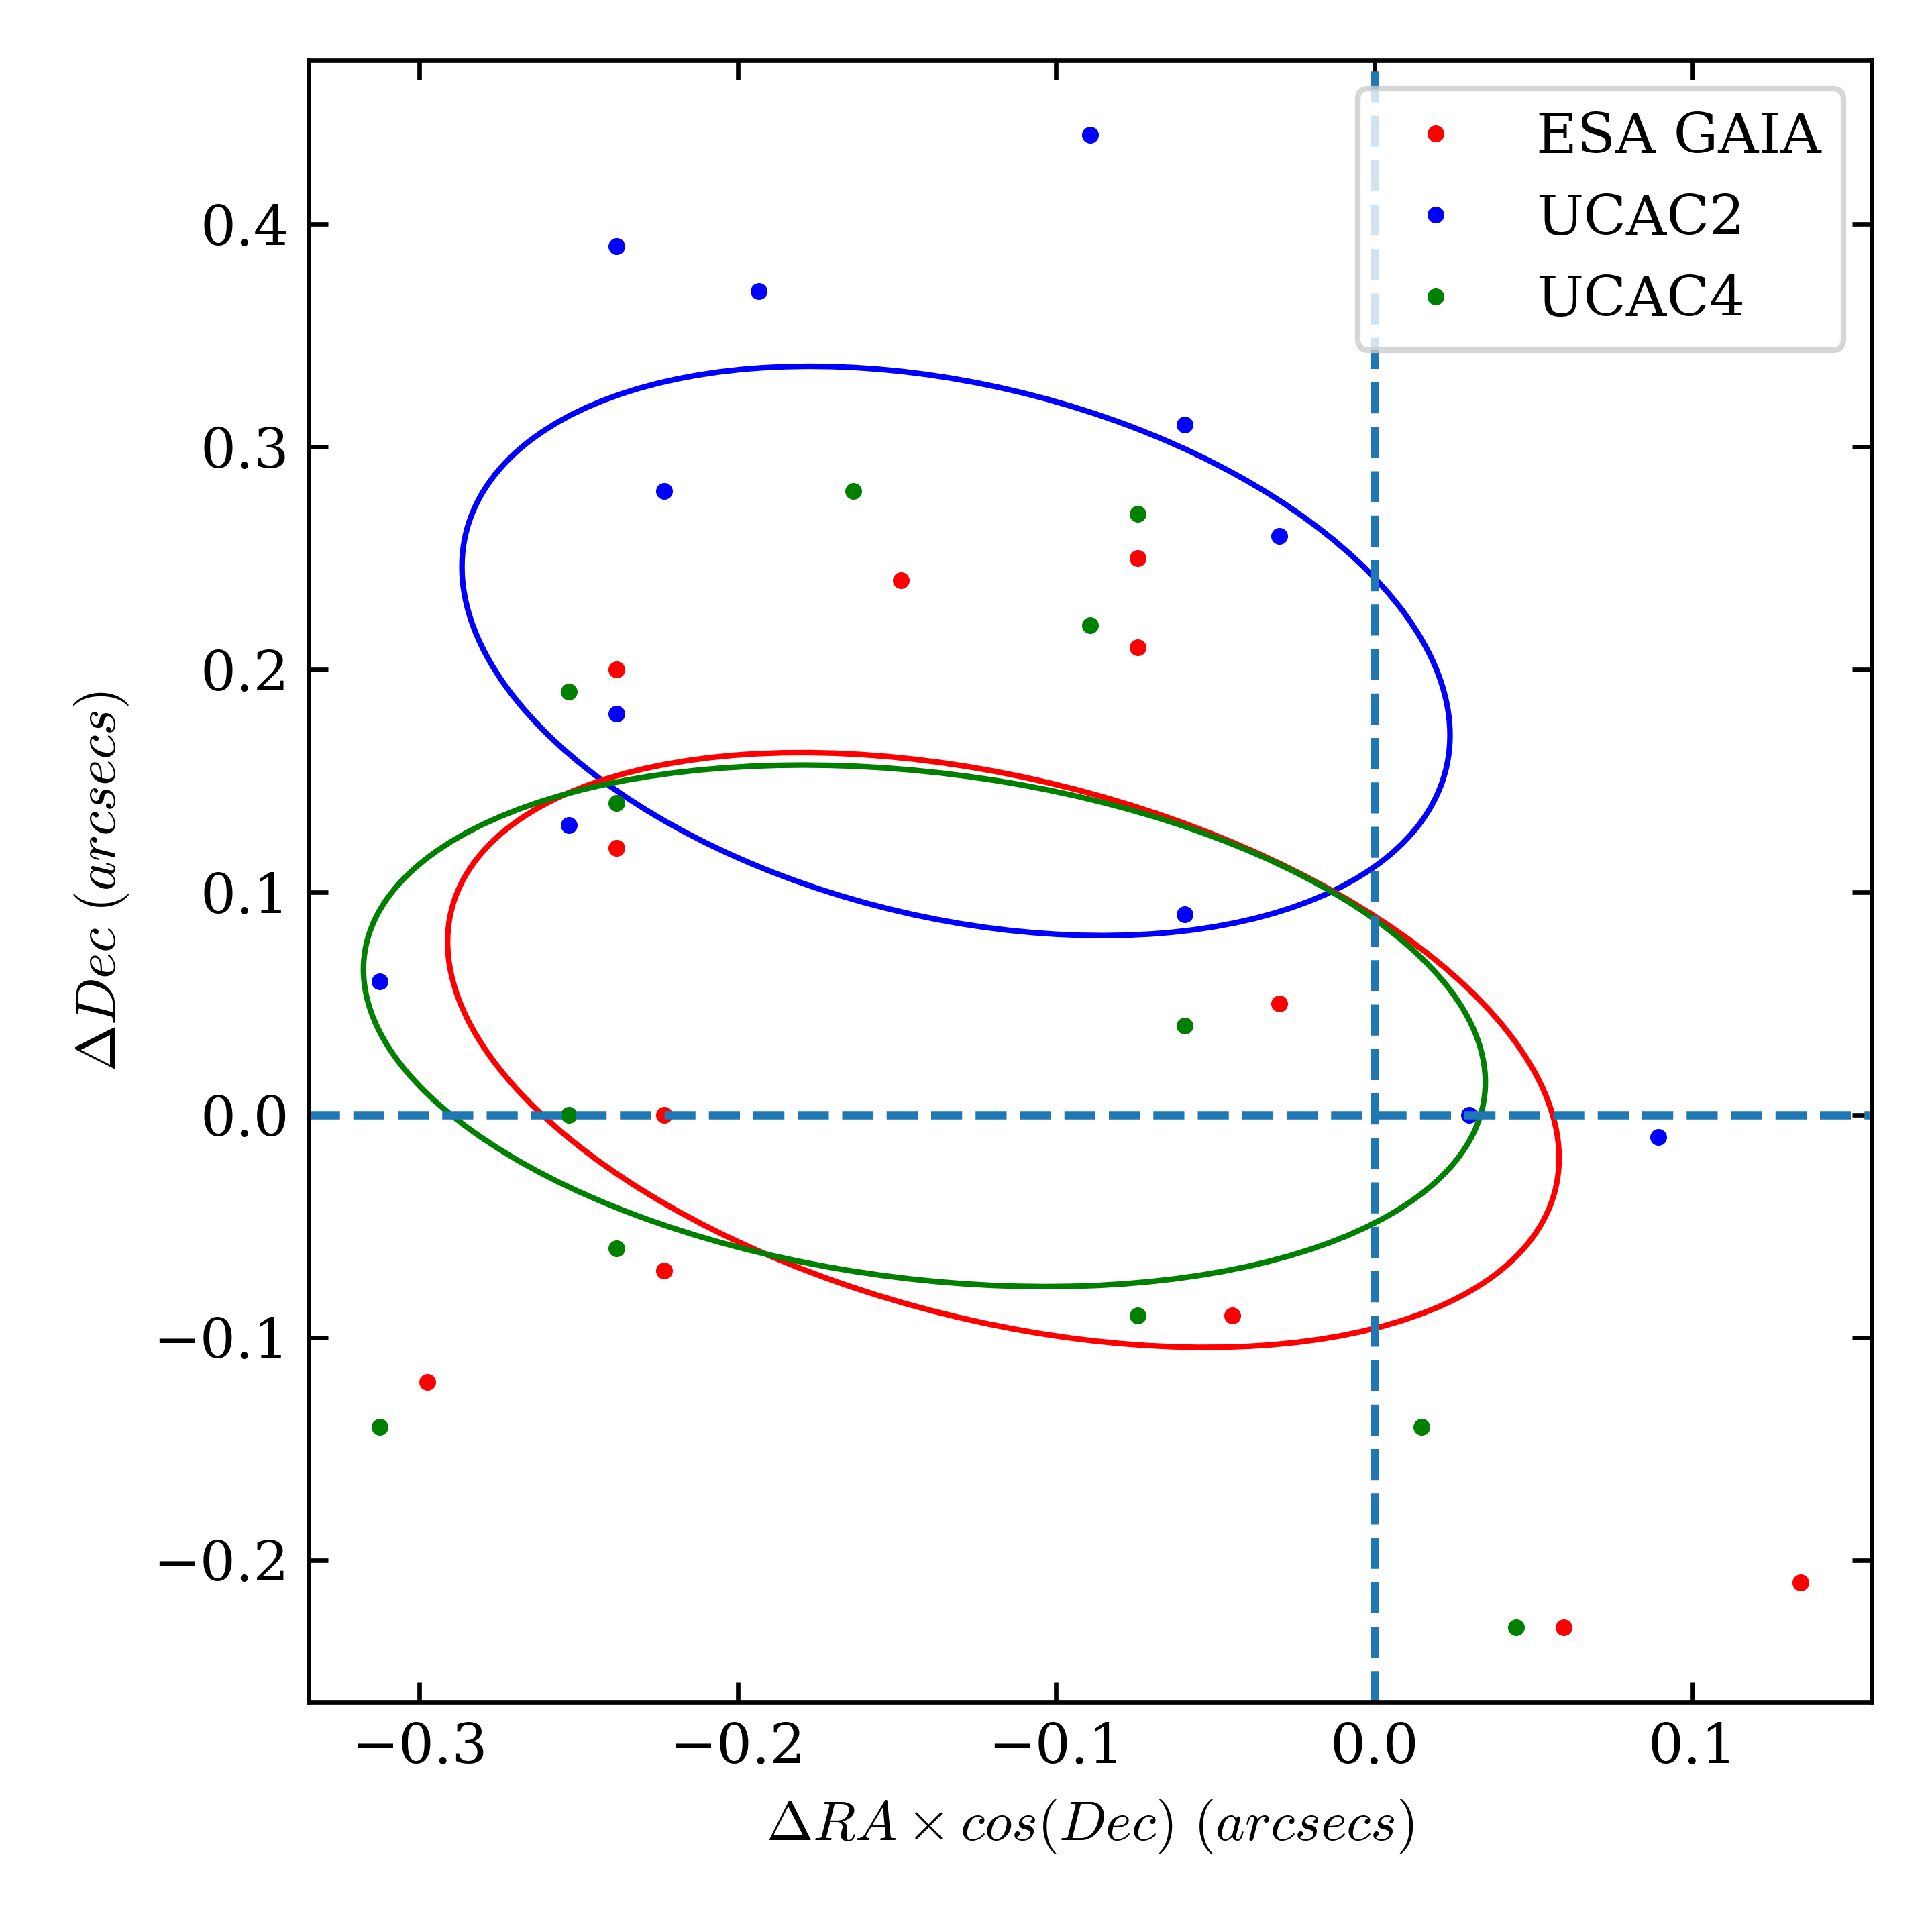
\includegraphics[width=0.5\textwidth]{20180424_174110_ASTROM_COMPARE}
\caption{The difference in $Dec.$ and $RA\cos(Dec)$ between the JPL HORIZONS ephemeris and a sample of 12 observations of Anchises using astrometry solutions from the UCAC2 (blue), UCAC4 (green) and GAIA (red) star catalogues. The $1\sigma$ error ellipse is shown for all catalogues. The zero point of both axes is shown as a dashed line, for reference.}
\label{fig: astrom compare}
\end{figure}

\begin{table}[h!]
\centering
\begin{tabularx}{0.5\textwidth}{ Y Y Y }
\hhline{===}
Catalogue & Mean $\Delta RA \cos (Dec)$ (arcsecs) & Mean $\Delta Dec$ (arcsecs) \\[3pt] \hline
UCAC2 & $-0.1 \pm 0.1$ & $0.2 \pm 0.1$ \\[3pt]
UCAC4 & $-0.1 \pm 0.1$ & $0.0 \pm 0.2$ \\[3pt]
GAIA & $-0.1 \pm 0.1$ & $0.0 \pm 0.2$ \\[3pt] \hline
\end{tabularx}
\caption{The mean $\Delta RA \cos (Dec)$ and mean $\Delta Dec$ for the UCAC2, UCAC4 and GAIA star catalogues compared to the JPL HORIZONS epehermis for twelve observations of Anchises. The errors displayed displayed are the $1\sigma$ root mean square (RMS) error.}
\label{tab: astrom compare results}
\end{table}


\subsection*{Orbit Determination}

To determine the orbits of each asteroid, their RAs and Decs. were measured using the astrometric solution from the UCAC4 catalogue. We then used our results with the Gauss method of determining orbits to calculate their orbital parameters.

The Gauss method is described in detail by Gronchi (2004) and is expanded on by Mitorabi (2014) who details how it can be adjusted from using only $3$ observations to using $N$ observations. This is more appropriate for our investigation as we are able to take numerous observations over a period of $7$ weeks which should improve the accuracy of our results. An outline of the algorithm for three observations described in ``Orbital Mechanics for Engineering Students''\scite{CurtisOrbitalmechanicsengineering2008} is given below:

\vspace{1ex}
The orbital parameters can be calculated from the Right Ascension, $\alpha_i$, and Declination, $\delta_i$, of three observations and also using the observer's position, $\mathbf{R}_i$, at the times of these observations and the times, $t_i$, of these observations where $i=1,2,3$ corresponds to each distinct observation. This algorithm begins by using the slant range unit vector, defined as $\mathbf{\hat{Q}}_i = \cos\delta_i \cos\alpha_i \mathbf{\hat{I}} + \cos\delta_i \sin\alpha_i \mathbf{\hat{J}} + \sin \delta_i \mathbf{\hat{K}}$ where $\mathbf{\hat{I},\hat{J},\hat{K}}$ are the heliocentric unit vectors. The algorithm then proceeds as:
\begin{enumerate}
 \item Calculate the time intervals between observations using the following:
 \begin{equation}
 \tau_1 = t_1 - t_2, \hspace{10pt} \tau_3 = t_3 - t_2, \hspace{10pt} \tau = \tau_3 - \tau_1.
 \end{equation}
 \item Calculate the cross products: 
 \begin{equation}
 \mathbf{p}_1 = \mathbf{\hat{Q}}_2 \times \mathbf{\hat{Q}}_3, \hspace{10pt} \mathbf{p}_2 = \mathbf{\hat{Q}}_1 \times \mathbf{\hat{Q}}_3, \hspace{10pt} \mathbf{p}_3 = \mathbf{\hat{Q}}_1 \times \mathbf{\hat{Q}}_2.
 \end{equation}
 \item Calculate $D_0 = \mathbf{\hat{Q}}_1 \cdot \mathbf{p}_1$.
 \item Calculate the 9 scalar quantities $D_{ij},\ i,j=1,2,3$ where $D_{ij}$ is defined by:
 \begin{equation}
 D_{ij} = \mathbf{R}_i \cdot \mathbf{p}_j.
 \end{equation} 
 \item Calculate the quantities $A$ and $B$ given by:
 \begin{equation}
 A = \frac{1}{D_0}\left(-D_{12}\frac{\tau_3}{\tau} +D_{22} + D_{32} \frac{\tau_1}{\tau} \right),
 \end{equation}
 \begin{equation}
 B = \frac{1}{6D_0} \left(D_{12}(\tau^2_3 - \tau^2)\frac{\tau_3}{\tau} + D_{32}(\tau^2 - \tau_1^2)\frac{\tau_1}{\tau}\right).
 \end{equation}
 \item Calculate the quantity, $E = \mathbf{R}_2 \cdot \mathbf{\hat{Q}}_2$.
 \item Calculate the quantities $a,\ b,\ c$ using $R_2^2 = \mathbf{R}_2 \cdot \mathbf{R}_2$, $\mu=GM$ where $G$ is Newton's universal gravitational constant and $M$ is the mass of the body being orbited, and the equations:
 \begin{equation}
 a = -(A^2 + 2AE + R_2^2),
 \end{equation}
 \begin{equation}
 b = -2\mu B(A+E),
 \end{equation}
 \begin{equation}
 c = -\mu^2B^2.
 \end{equation}
 \item Find the roots of the equation:
 \begin{equation}
 x^8 + ax^6 +bx^3 +c = 0,
 \end{equation}
 with the most physically reasonable root equalling $r_2$. If more than one root seems appropriate, store them and continue the algorithm on all viable roots in parallel, comparing the final calculated orbital parameters to the literature to determine the correct solution.
 \item Calculate $Q_2 = A + \mu B/r_2^3$ and $Q_1$ and $Q_3$ using the following:
 \begin{multline} 
 Q_1 = \Bigg( \frac{6 \left(D_{31} \frac{\tau_1}{\tau_3} +D_{21}\frac{\tau}{\tau_3}\right) r^3_2 + \mu D_{31}(\tau^2 -\tau_1^2) \frac{\tau_1}{\tau_3} }{6r_2^3 + \mu(\tau^2-\tau^2_3)} \\
 -D_{11} \Bigg) \frac{1}{D_0} ,
 \end{multline}
 \begin{multline} 
 Q_3 = \Bigg( \frac{6 \left(D_{13} \frac{\tau_3}{\tau_1} -D_{23}\frac{\tau}{\tau_1}\right) r^3_2 + \mu D_{13}(\tau^2 - \tau_3^2) \frac{\tau_3}{\tau_31} }{6r_2^3 + \mu(\tau^2-\tau^2_3)} \\ 
 - D_{33} \Bigg)\frac{1}{D_0} .
 \end{multline}
 \item Calculate the $\mathbf{r}_i,\ i=1,2,3$ vectors using:
 \begin{equation}
 \mathbf{r_i} = \mathbf{R_i} + Q_i \mathbf{\hat{Q}}_i,
 \end{equation}
 where $\mathbf{r}_i\ i=1,2,3$ are the position vectors for the object at the time of the three observations used in this algorithm.
 \item Calculate $f_i,g_i,\ i=1,3$ using the equations:
 \begin{equation}
 f_i \approx 1 - \frac{1}{2}\frac{\mu}{r_2^3}\tau_i^2 ,
 \end{equation}
 \begin{equation}
 g_i \approx \tau_i - \frac{1}{6}\frac{\mu}{r_2^3}\tau_i^3 .
 \end{equation}
 \item Calculate $\mathbf{v}_2$ using the equation:
 \begin{equation}
 \mathbf{v}_2 = \frac{1}{f_1g_3-f_3g_1}(-f_3\mathbf{r}_1+f_1\mathbf{r}_3) ,
 \end{equation}
 where $\mathbf{v}_2$ is the velocity vector at the time of the second observation.
 \item Calculate the specific angular momentum, $\mathbf{h}$:
 \begin{equation}
 \mathbf{h} = \mathbf{r}_2 \times \mathbf{v}_2 .
 \end{equation} 
 \item Calculate the inclination using the z-component of $\mathbf{h}$, $h_z$:
 \begin{equation}
 i = \arccos\left( \frac{h_z}{|\mathbf{h}|} \right) .
 \end{equation}
 \item Calculate the vector that defines the node line, $N$, using:
 \begin{equation}
 \mathbf{N} = \mathbf{\hat{K}} \times \mathbf{h} .
 \end{equation} 
 \item Calculate the RA of the ascending node:
 \begin{equation}
 \Omega = \arccos \left( \frac{N_x}{|\mathbf{N}|} \right) ,
 \end{equation}
 where $N_x$ is the $x$ component of $\mathbf{N}$.
 \item Calculate the eccentricity vector, $\mathbf{e}$, using:
 \begin{equation}
 \mathbf{e} = \frac{1}{\mu} \left[ \left(\mathbf{v}^2 - \frac{\mu}{|\mathbf{r}|} \right) \mathbf{r} - (\mathbf{r}\cdot\mathbf{v}) \mathbf{v} \right] ,
 \end{equation}
 where the eccentricity orbital parameter, $e$, is given by $e = |\mathbf{e}|$.
 \item Calculate the argument of perigee, $\omega$, using:
 \begin{equation}
 \omega = \arccos \left( \frac{\mathbf{N} \cdot \mathbf{e}}{|\mathbf{N}||\mathbf{e}|} \right) .
 \end{equation}
 \item Calculate the true anomaly, $\nu$, using:
 \begin{equation}
 \nu = \arccos \left( \frac{\mathbf{e} \cdot \mathbf{r}}{|\mathbf{e}||\mathbf{r}|} \right) .
 \end{equation}
\end{enumerate}
From the parameters $\mathbf{h},\ i,\ \Omega,\ \omega,\ e,\ \nu,$ all other orbital parameters can be derived.
\vspace{1ex}

The implementation of the Gauss method we use is the Find\_Orb orbit determination software.\scite{FindOrbOrbit} To verify that this returns accurate results, we use RA and Decs. from an ephemeris generated by JPL HORIZONS and investigate if the calculated orbital parameters from Find\_Orb converge to the JPL result. We would expect this to happen if the software was functioning correctly. 

This analysis was first performed using an ephemeris of Patroclus for one observation per week for 13 weeks. This is approximately equal to the number of observations we took in this investigation over the same time frame. The results of this preliminary investigation are shown in Fig. \ref{fig: JPL-find orb convergence}.

These results show that, generally, Find\_Orb's solutions do converge to the JPL HORIZONS orbital parameters. However, the results are very noisy showing a large variance in the solutions being returned. This is most likely due to the observations being taken from a small arc of the orbit.

\begin{figure}[h!]
\centering
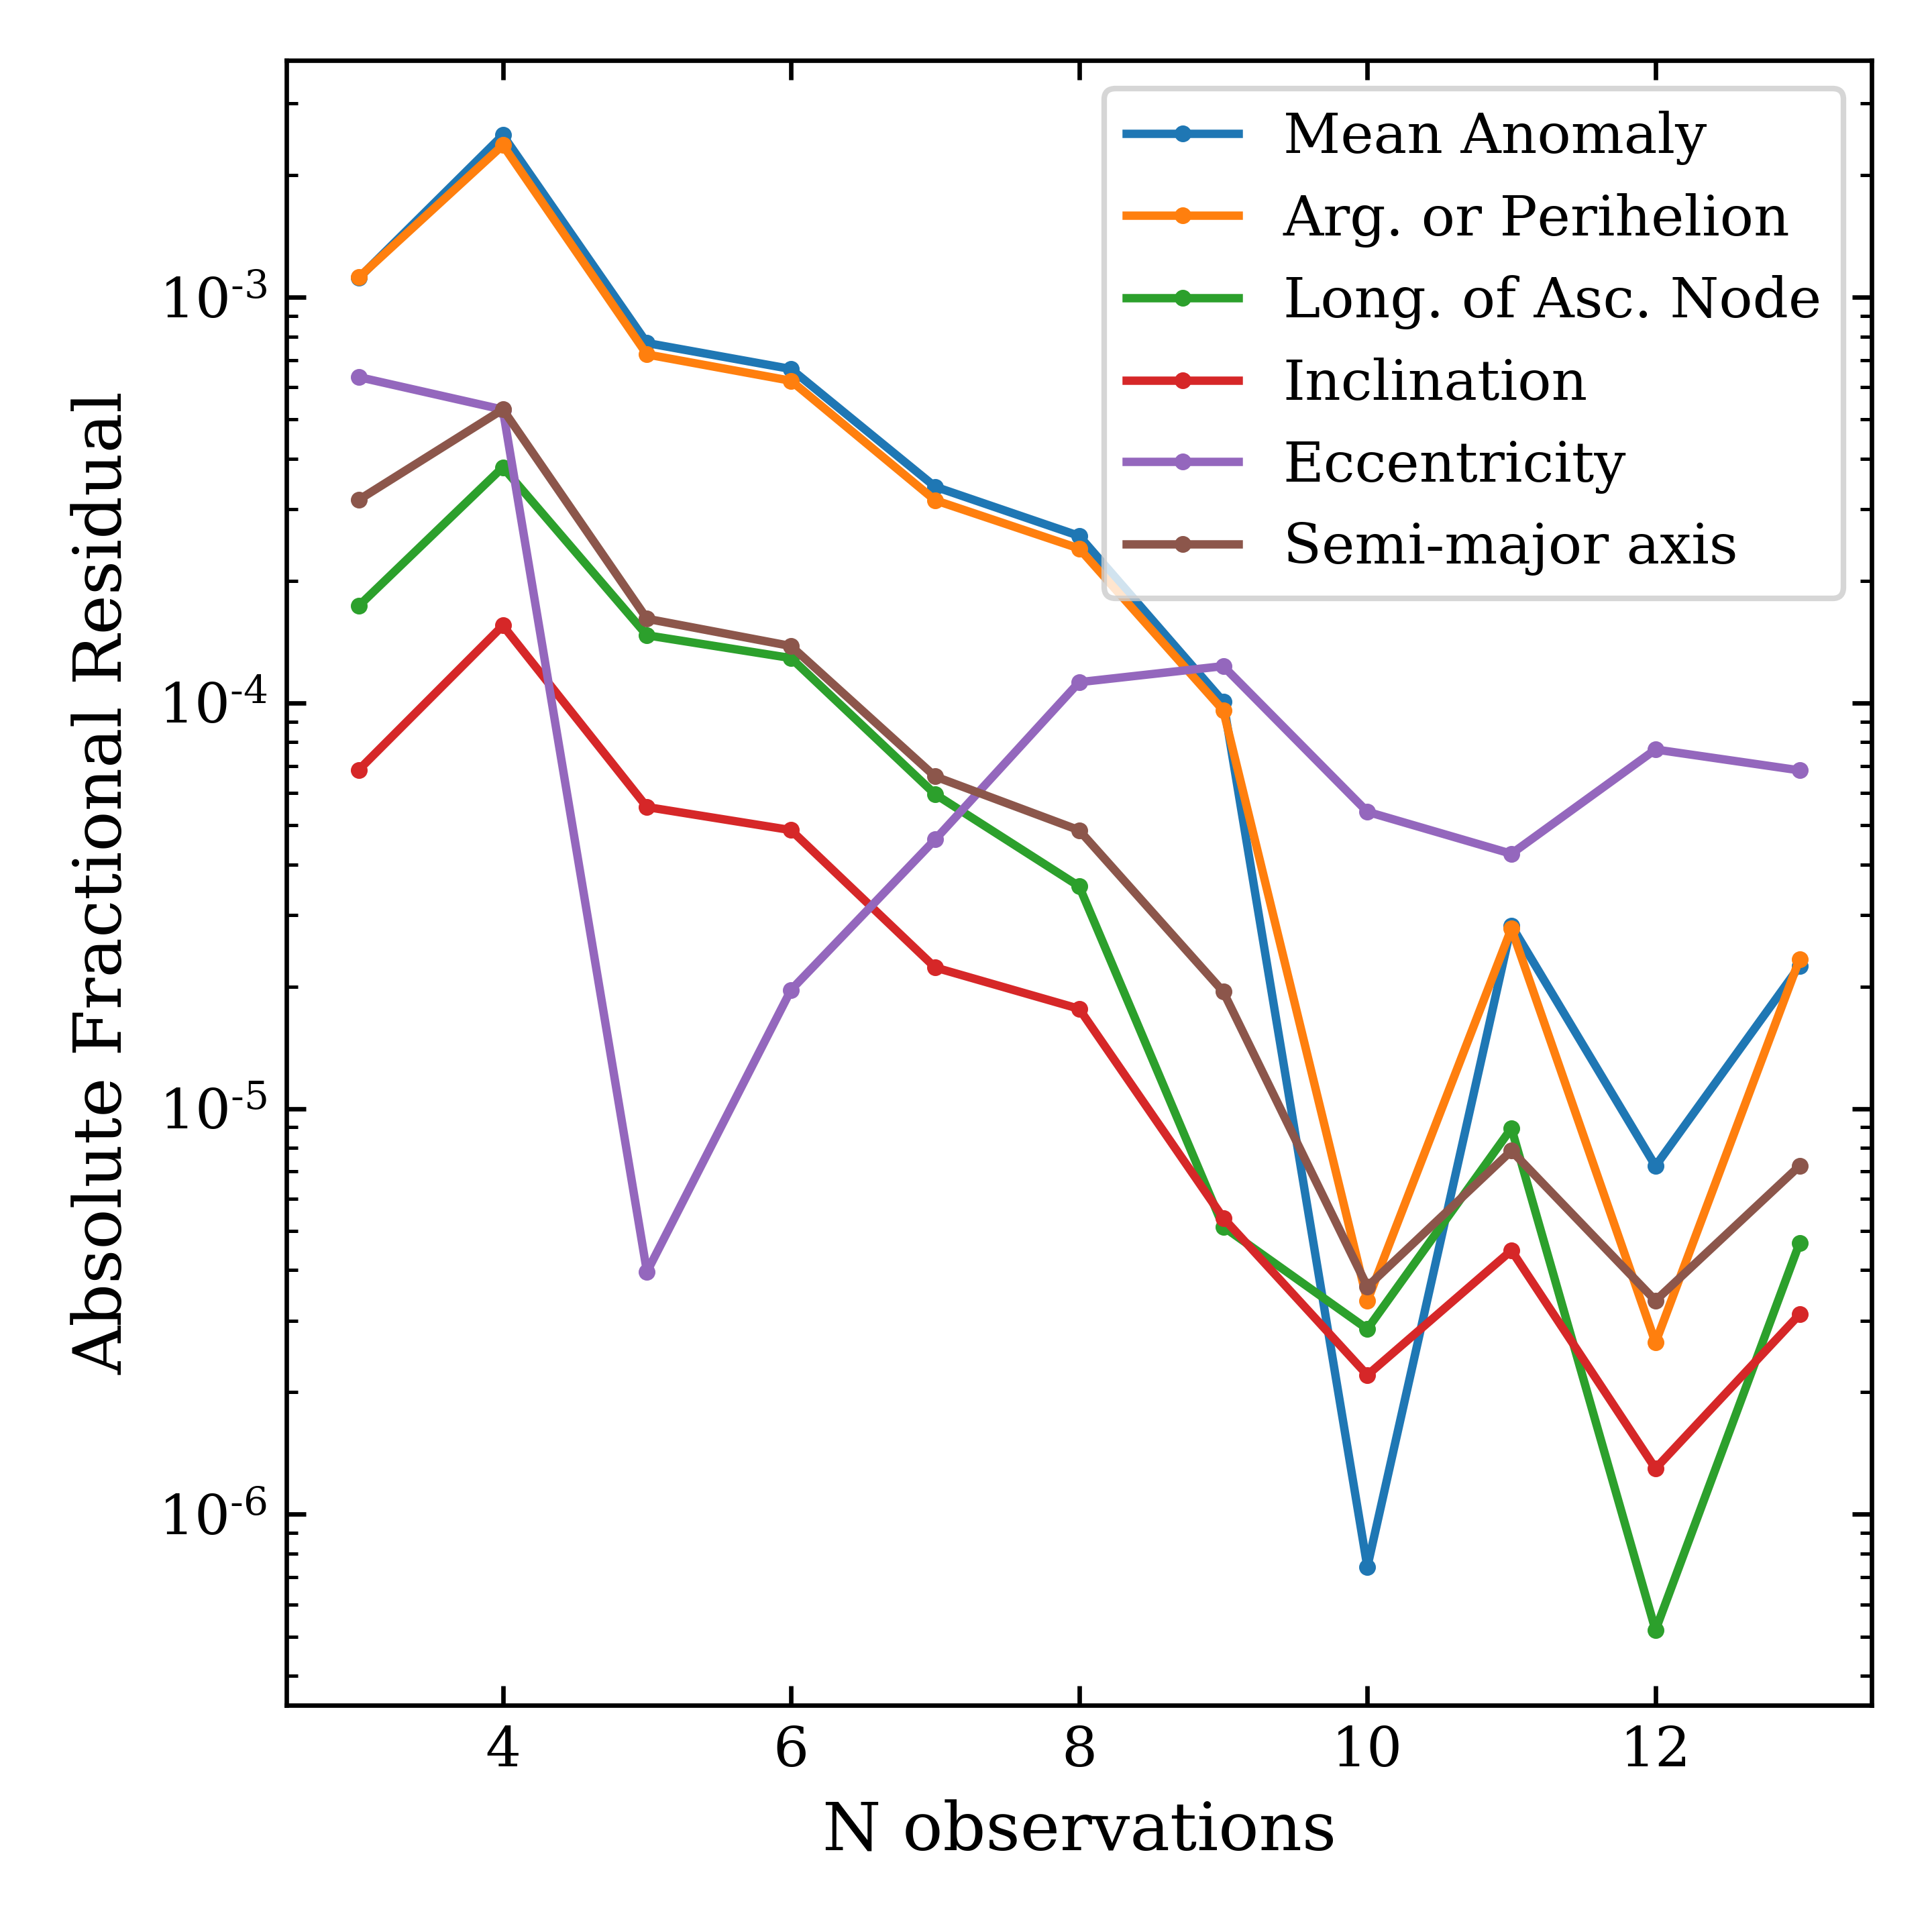
\includegraphics[width=0.5\textwidth]{20180424_205752_JPL_FINDORB_CONVERGENCE}
\caption{The absolute fractional residual between the Find\_Orb orbital parameters and the JPL HORIZONS parameters using an increasing number of ephemeris observation points over 13 weeks.}
\label{fig: JPL-find orb convergence}
\end{figure}

To investigate the effect of a greater arc of observations and to see if this improves convergence, this investigation was performed again. However, the observations were taken from the JPL HORIZONS ephemeris for one observation per month for 18 months and excluding those that would be below the horizon in Durham.
\begin{figure}[h!]
\centering
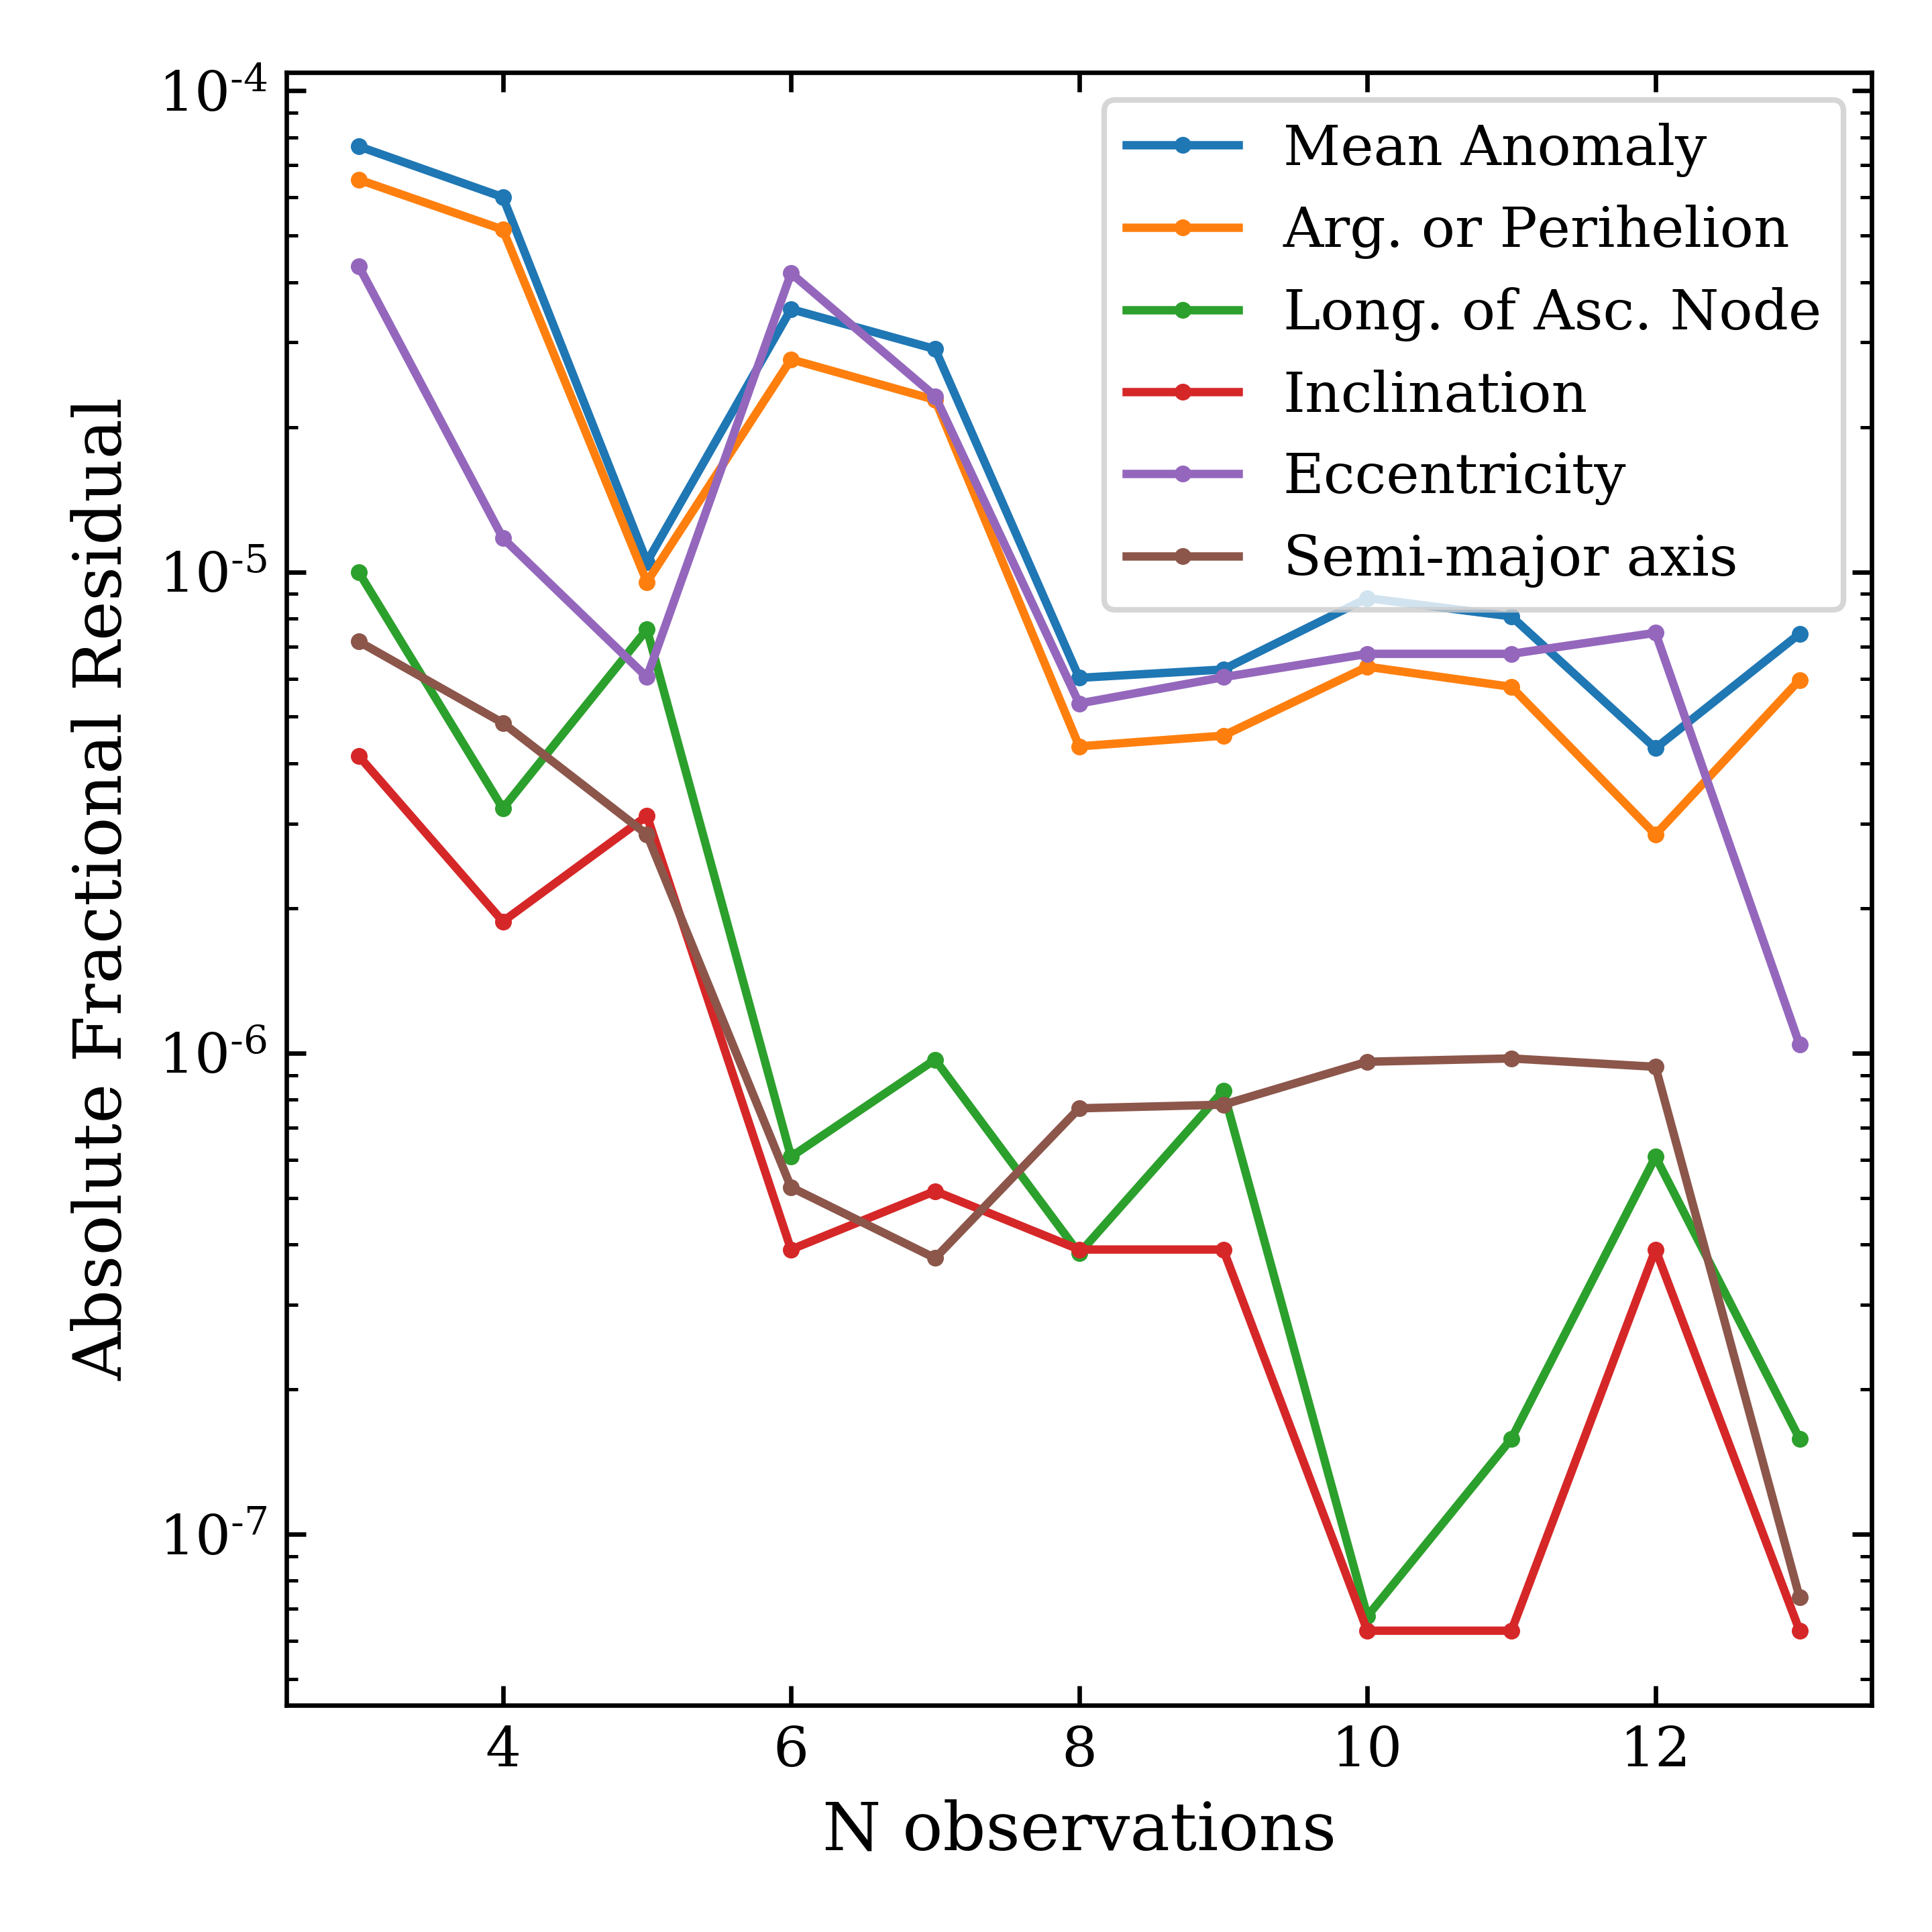
\includegraphics[width=0.5\textwidth]{20180424_205806_JPL_FINDORB_CONVERGENCE}
\caption{The absolute fractional residual between the Find\_Orb orbital parameters and the JPL HORIZONS parameters using an increasing number of ephemeris observation points over 18 months.}
\label{fig: JPL-find orb convergence 18mth}
\end{figure}

Fig. \ref{fig: JPL-find orb convergence 18mth} shows that the convergence to the literature values is greater and faster when using observations taken from a greater arc length of the orbit, as in this case all parameters reach a a fractional residual $<10^{-5}$ after 8 observations; this does not happen for the shorter arc of observations. These results show that using observations covering a longer time frame produce more accurate results. Therefore, in this investigation we couple our own observations with archival data. Both Fig. \ref{fig: JPL-find orb convergence} and Fig. \ref{fig: JPL-find orb convergence 18mth} show that a good level of convergence can be found using the Find\_Orb software and this implementation would be suitable for this investigation.

We proceeded with using Find\_Orb to determine the orbital parameters of our asteroids. To supplement our observations of Patroclus and Priamus, archival data was acquired. For Patroclus, 9 further observations from 2001 to 2017 and for Priamus, 5 further observations from 2011 to 2016 were acquired and used to improve the accuracy and error confidence in the calculated orbital parameters.

The errors on the orbital parameters were calculated using a jackknifing method: assuming we have N observations, we systematically remove one observation from the data set, we then calculate and keep a record of the orbital parameters on this set of $N-1$ observations. This is repeated until every observation has been removed once. We then have  a distribution for each orbital parameter that is fit to a gaussian where the mean is the orbital parameter of the population and the standard deviation is the error on that parameter. In this investigation, all quoted errors represent the $1\sigma$ uncertainty unless otherwise stated.

\subsection*{Positional Prediction}

Once the orbital parameters had been acquired, they were used to predict the position of the asteroid at any given time. This is not trivial as it must take account of the osculating orbit, as previously discussed.

We used the Pyephem python package with the calculated orbital parameters and epochs to determine the position of the asteroid at a given time. The specific algorithms are described in detail by Peter Duffett-Smith and Jonathan Zwart in ``Practical Astronomy with your Calculator or Spreadsheet.''\textsuperscript{\cite[p.121-130]{Duffett-SmithPracticalastronomyyour2011}} An outline of the method to calculate the heliocentric position is given here:

\vspace{1ex}
The heliocentric Cartesian coordinates, $x,\ y,\ z$, can calculated from a body's Keplerian orbital parameters.
\begin{enumerate}
\item Numerically solve the following equation for the eccentric anomaly, $E$, from the mean anomaly, $M$, and eccentricity, $e$:
\begin{equation}
M = E - e \sin E .
\end{equation}
\item Calculate the true anomaly, $\nu$, from the eccentric anomaly and eccentricity using the equation:
\begin{equation}
\tan \frac{\nu}{2} = \left(\frac{1+e}{1-e} \right)^{1/2} \tan \frac{E}{2} .
\end{equation}
\item Calculate the radial distance, $r$, from the semi-major axis, $a$, using the equation:
\begin{equation}
r = a(1-e\cos E) .
\end{equation}
\item Calculate the $x,\ y,\ z$ coordinates using the equations:
\begin{equation} \label{eq: xpos}
x = r(\cos\Omega\cos(\omega+\nu) - \sin\Omega\sin(\omega+\nu)\cos i) ,
\end{equation}
\begin{equation} \label{eq: ypos}
y = r(\sin\Omega\cos(\omega+\nu) + \cos\Omega\sin(\omega+\nu)\cos i) ,
\end{equation}
\begin{equation} \label{eq: zpos}
z = r\sin i \sin(\omega+\nu) .
\end{equation}
\end{enumerate}
Equations (\ref{eq: xpos}), (\ref{eq: ypos}) and (\ref{eq: zpos}) define the heliocentric coordinate position of the asteroid with the $x$-axis direction based on the epoch of the mean anomaly and in the plane of the ecliptic, the $y$-axis perpendicular to the $x$ axis in the plane of the ecliptic and the $z$-axis normal to the ecliptic.
\vspace{1ex}

The errors on the orbital parameters are propagated through to the calculated position by generating a sample of orbital parameters that are perturbed by a random Gaussian distribution with the mean as the orbital parameter and standard deviation equal to the error on the orbital parameter. Positions can then be calculated from this randomised sample, producing a distribution of positions for the asteroid. The error in each Cartesian direction is then given by the square root of the diagonal elements of the covariance matrix of this position distribution. We generate an error ellipsoid from this distribution using the eigenvalues and eigenvectors of the covariance matrix where the roots of the eigenvalues give the error in each direction of the basis defined by the eigenvectors. The roots of the eigenvalues are used as the principal semi-axes of the ellipsoid. The volume of the ellipsoid gives the confidence volume, the volume of an ellipsoid, $V$, is given by:
\begin{equation} \label{eq: v ellipsoid}
V = \frac{4}{3}\pi a b c ,
\end{equation}
where $a,\ b,\ c$ are the principal semi-axes lengths and are equal to the root of the eigenvalues of the covariance matrix.

\subsection*{Orbital Transfer}

Once the position of the asteroid has been determined, the possible orbital transfers to the asteroid can be investigated. For this investigation we assume that the \textit{Lucy} spacecraft will perform a Hohmann transfer from a parking orbit at the Earth's heliocentric radius to the asteroid's predicted position, within the plane of the asteroid's orbit. 

A Hohmann transfer assumes an initial circular parking orbit in the plane of the target orbit. It consists of two instantaneous burns. The first takes the initial circular orbit to an elliptical orbit with its apoapsis at the radius of the target orbit. The second burn then occurs at the apoapsis of the elliptical orbit to convert the elliptical orbit to the target orbit. Fig. \ref{fig: hohmann trasnfer} shows an illustration of the Hohmann transfer orbit, where $\Delta v_1$ and $\Delta v_2$ represent the first and second burns respectively.

\begin{figure}[h!]
\centering
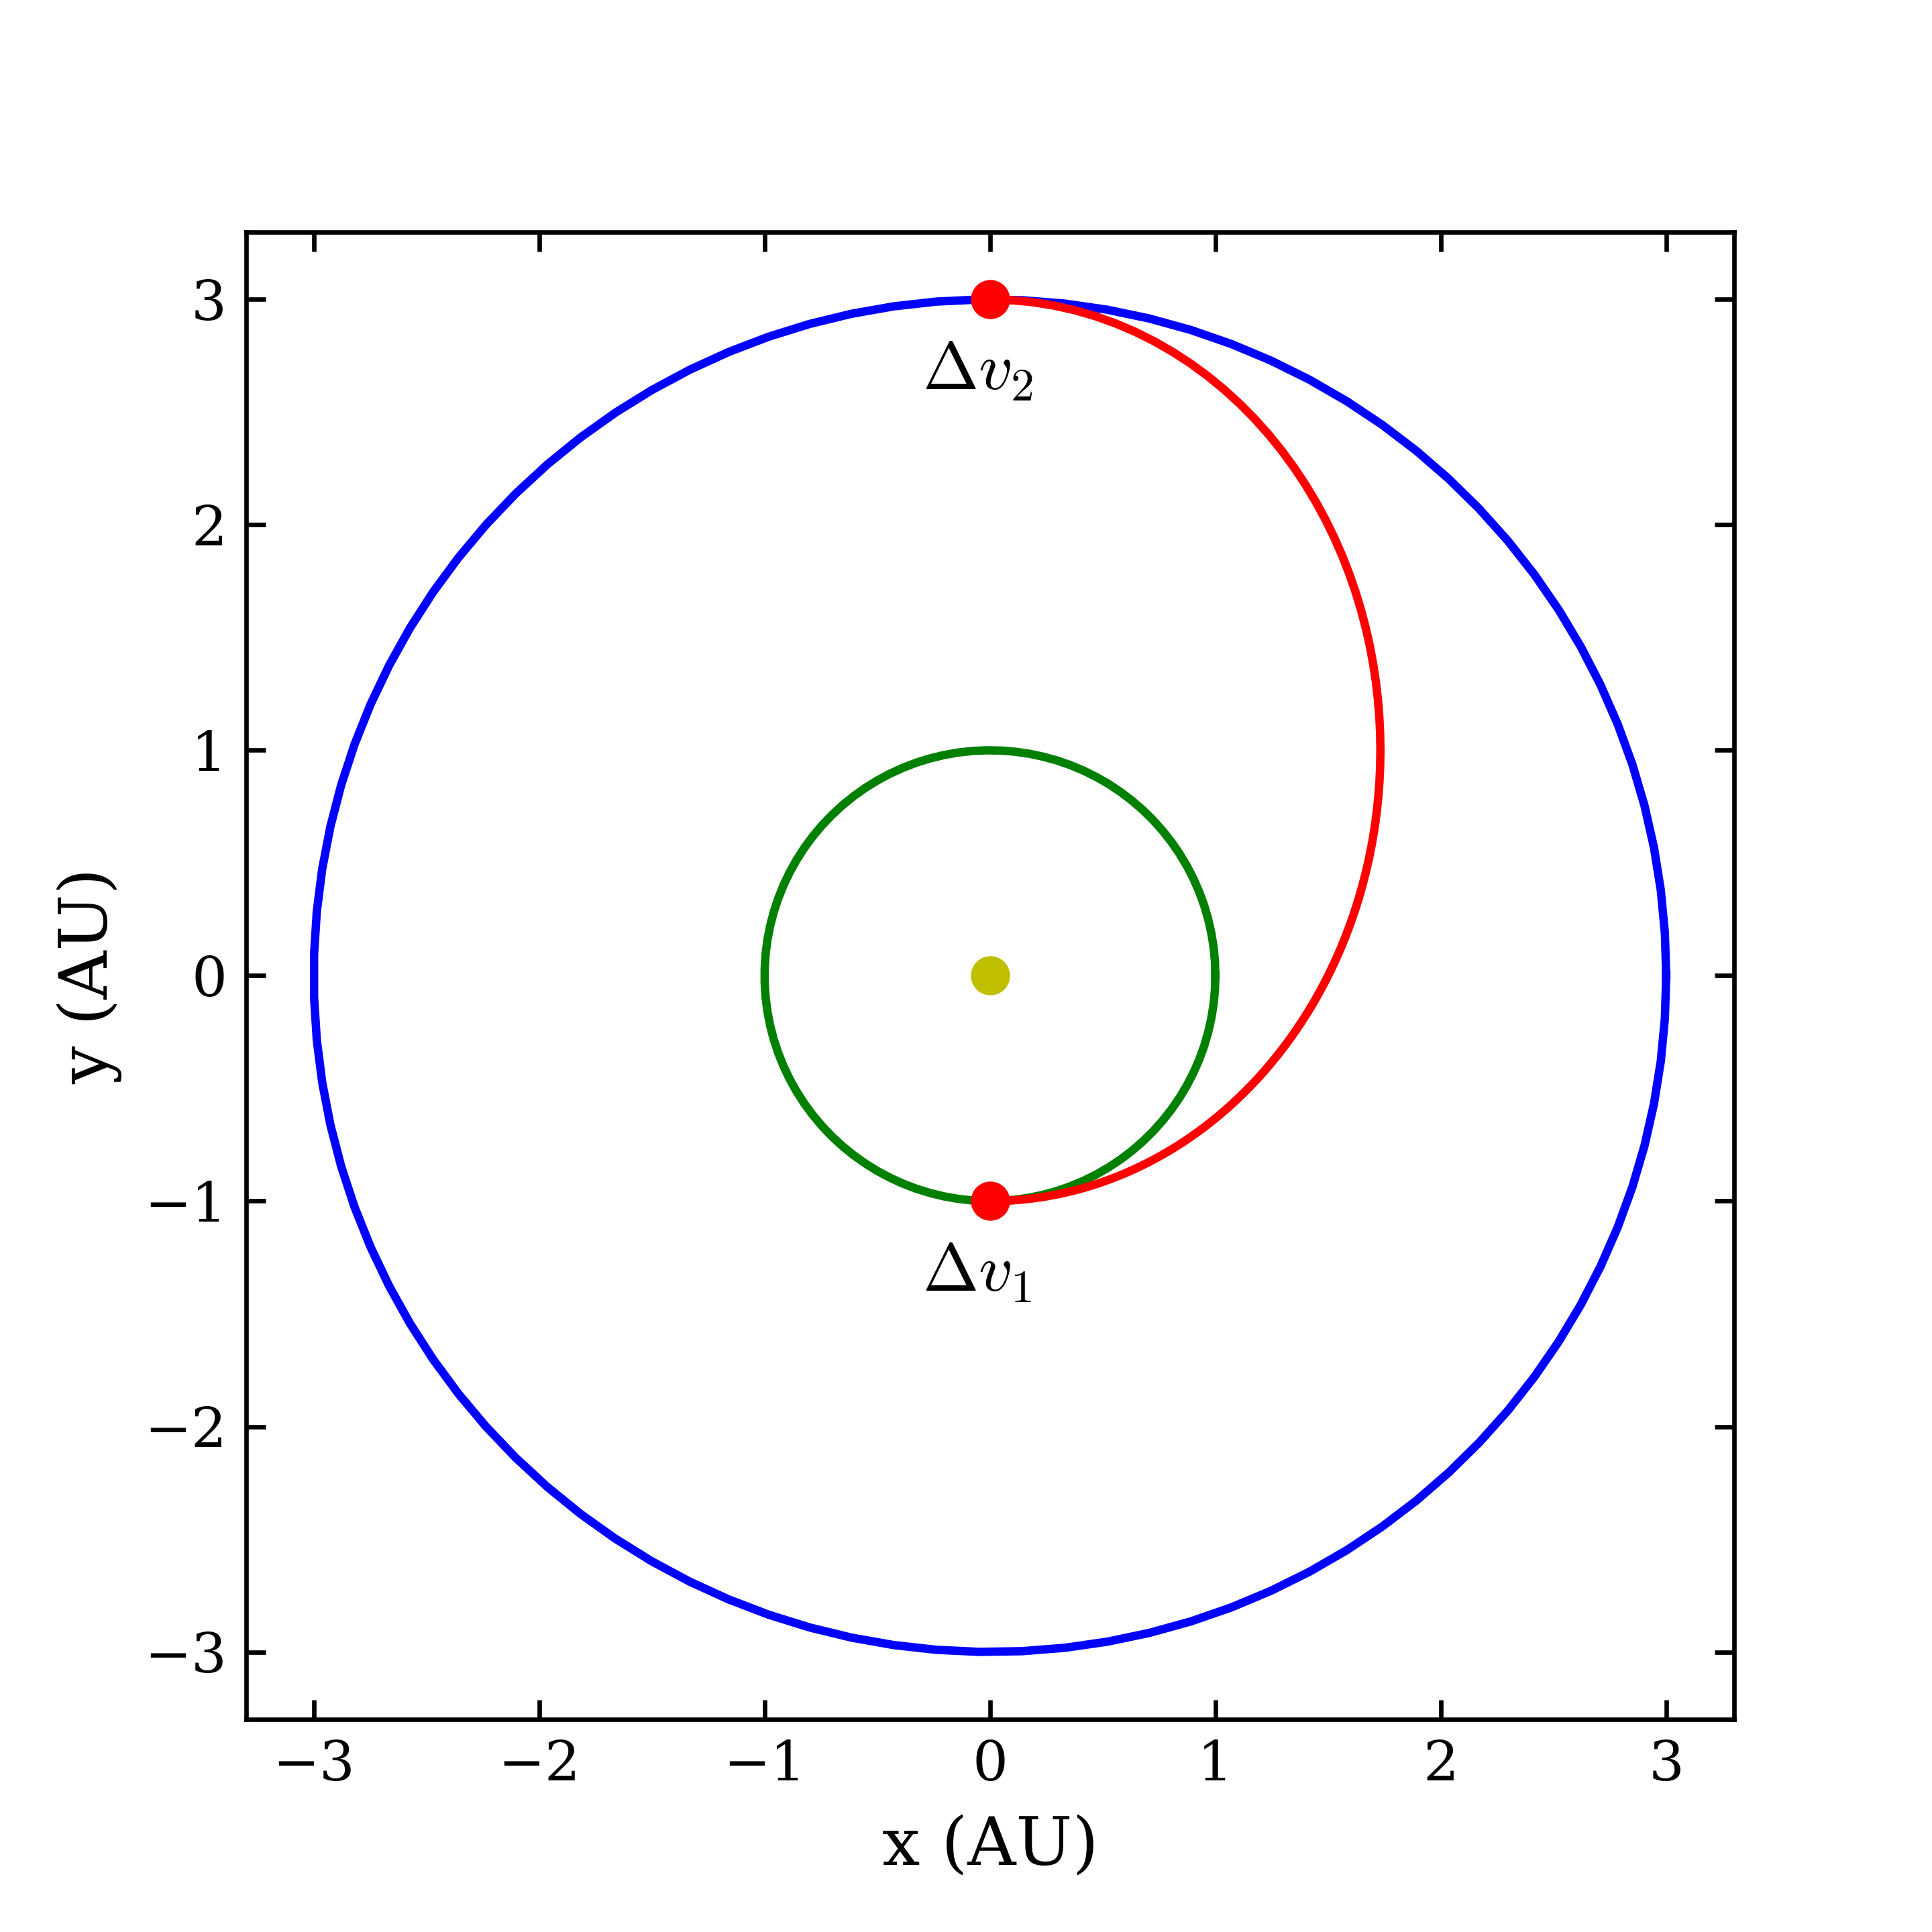
\includegraphics[width=0.5\textwidth]{20180410_200052_HOHMANN_TRANSFER_EXAMPLE}
\caption{The green and blue lines represent circular orbits around the Sun (yellow point) with radii equal to 1 and 3 AU respectively. The red line represents the Hohmann transfer. The burn positions are marked with red points and text. The $\Delta v$ requirement of each burn are given in Equations (\ref{eq: delta v1}) and (\ref{eq: delta v2}).}
\label{fig: hohmann trasnfer}
\end{figure}

The change in velocity required to achieve these orbits is given by the following equations:
\begin{equation} \label{eq: delta v1}
\Delta v_1 = \sqrt{\frac{\mu}{r_1}}\left( \sqrt{\frac{2r_2}{r_1+r_2}}-1 \right),
\end{equation} 
\begin{equation} \label{eq: delta v2}
\Delta v_2 = \sqrt{\frac{\mu}{r_2}}\left( 1- \sqrt{\frac{2r_1}{r_1+r_2}} \right),
\end{equation} 
where $r_1$ is the radius of the inner orbit, $r_2$ is the radius of the outer orbit and $\mu = GM$ where $G$ is Newton's gravitational constant and $M$ is the mass of the body being orbited, in our case the Sun. The total velocity change required by the Hohmann transfer, $\Delta v_{T}$, is given trivially by the sum of $\Delta v_1$ and $\Delta v_2$.

Using our calculated positions for Patroclus, we find the maximum and minimum radii of the $1\sigma$ error ellipsoid. We then use Equations (\ref{eq: delta v1}) and (\ref{eq: delta v2}) to calculate the range in $\Delta v_{T}$ due to the uncertainty in Patroclus' calculated position. For the \textit{Lucy} mission, we place an upper bound on the $\Delta v_{T}$ requirement in order to reduce the fuel requirement and hence the mass of the spacecraft.

Modelling the orbital transfer to Patroclus as a Hohmann transfer from a parking orbit at Earth's radius is a simplification to the flight plan originally suggested for the \textit{Lucy} mission, \textit{Lucy} will first fly to the L4 camp of Trojan asteroids before switching to Patroclus in the L5 camp using a complex set of orbital manoeuvres.\scite{47thLunarPlanetary} However, this simplified orbital transfer will highlight the difference in $\Delta v$ requirements from increasing the confidence in the calculated position for Patroclus.

\section{Results} 

The observations acquired in this investigation from 24th January 2018 to 10th March 2018 are shown in Fig. \ref{fig: observations}.

\begin{figure}[h!]
\centering
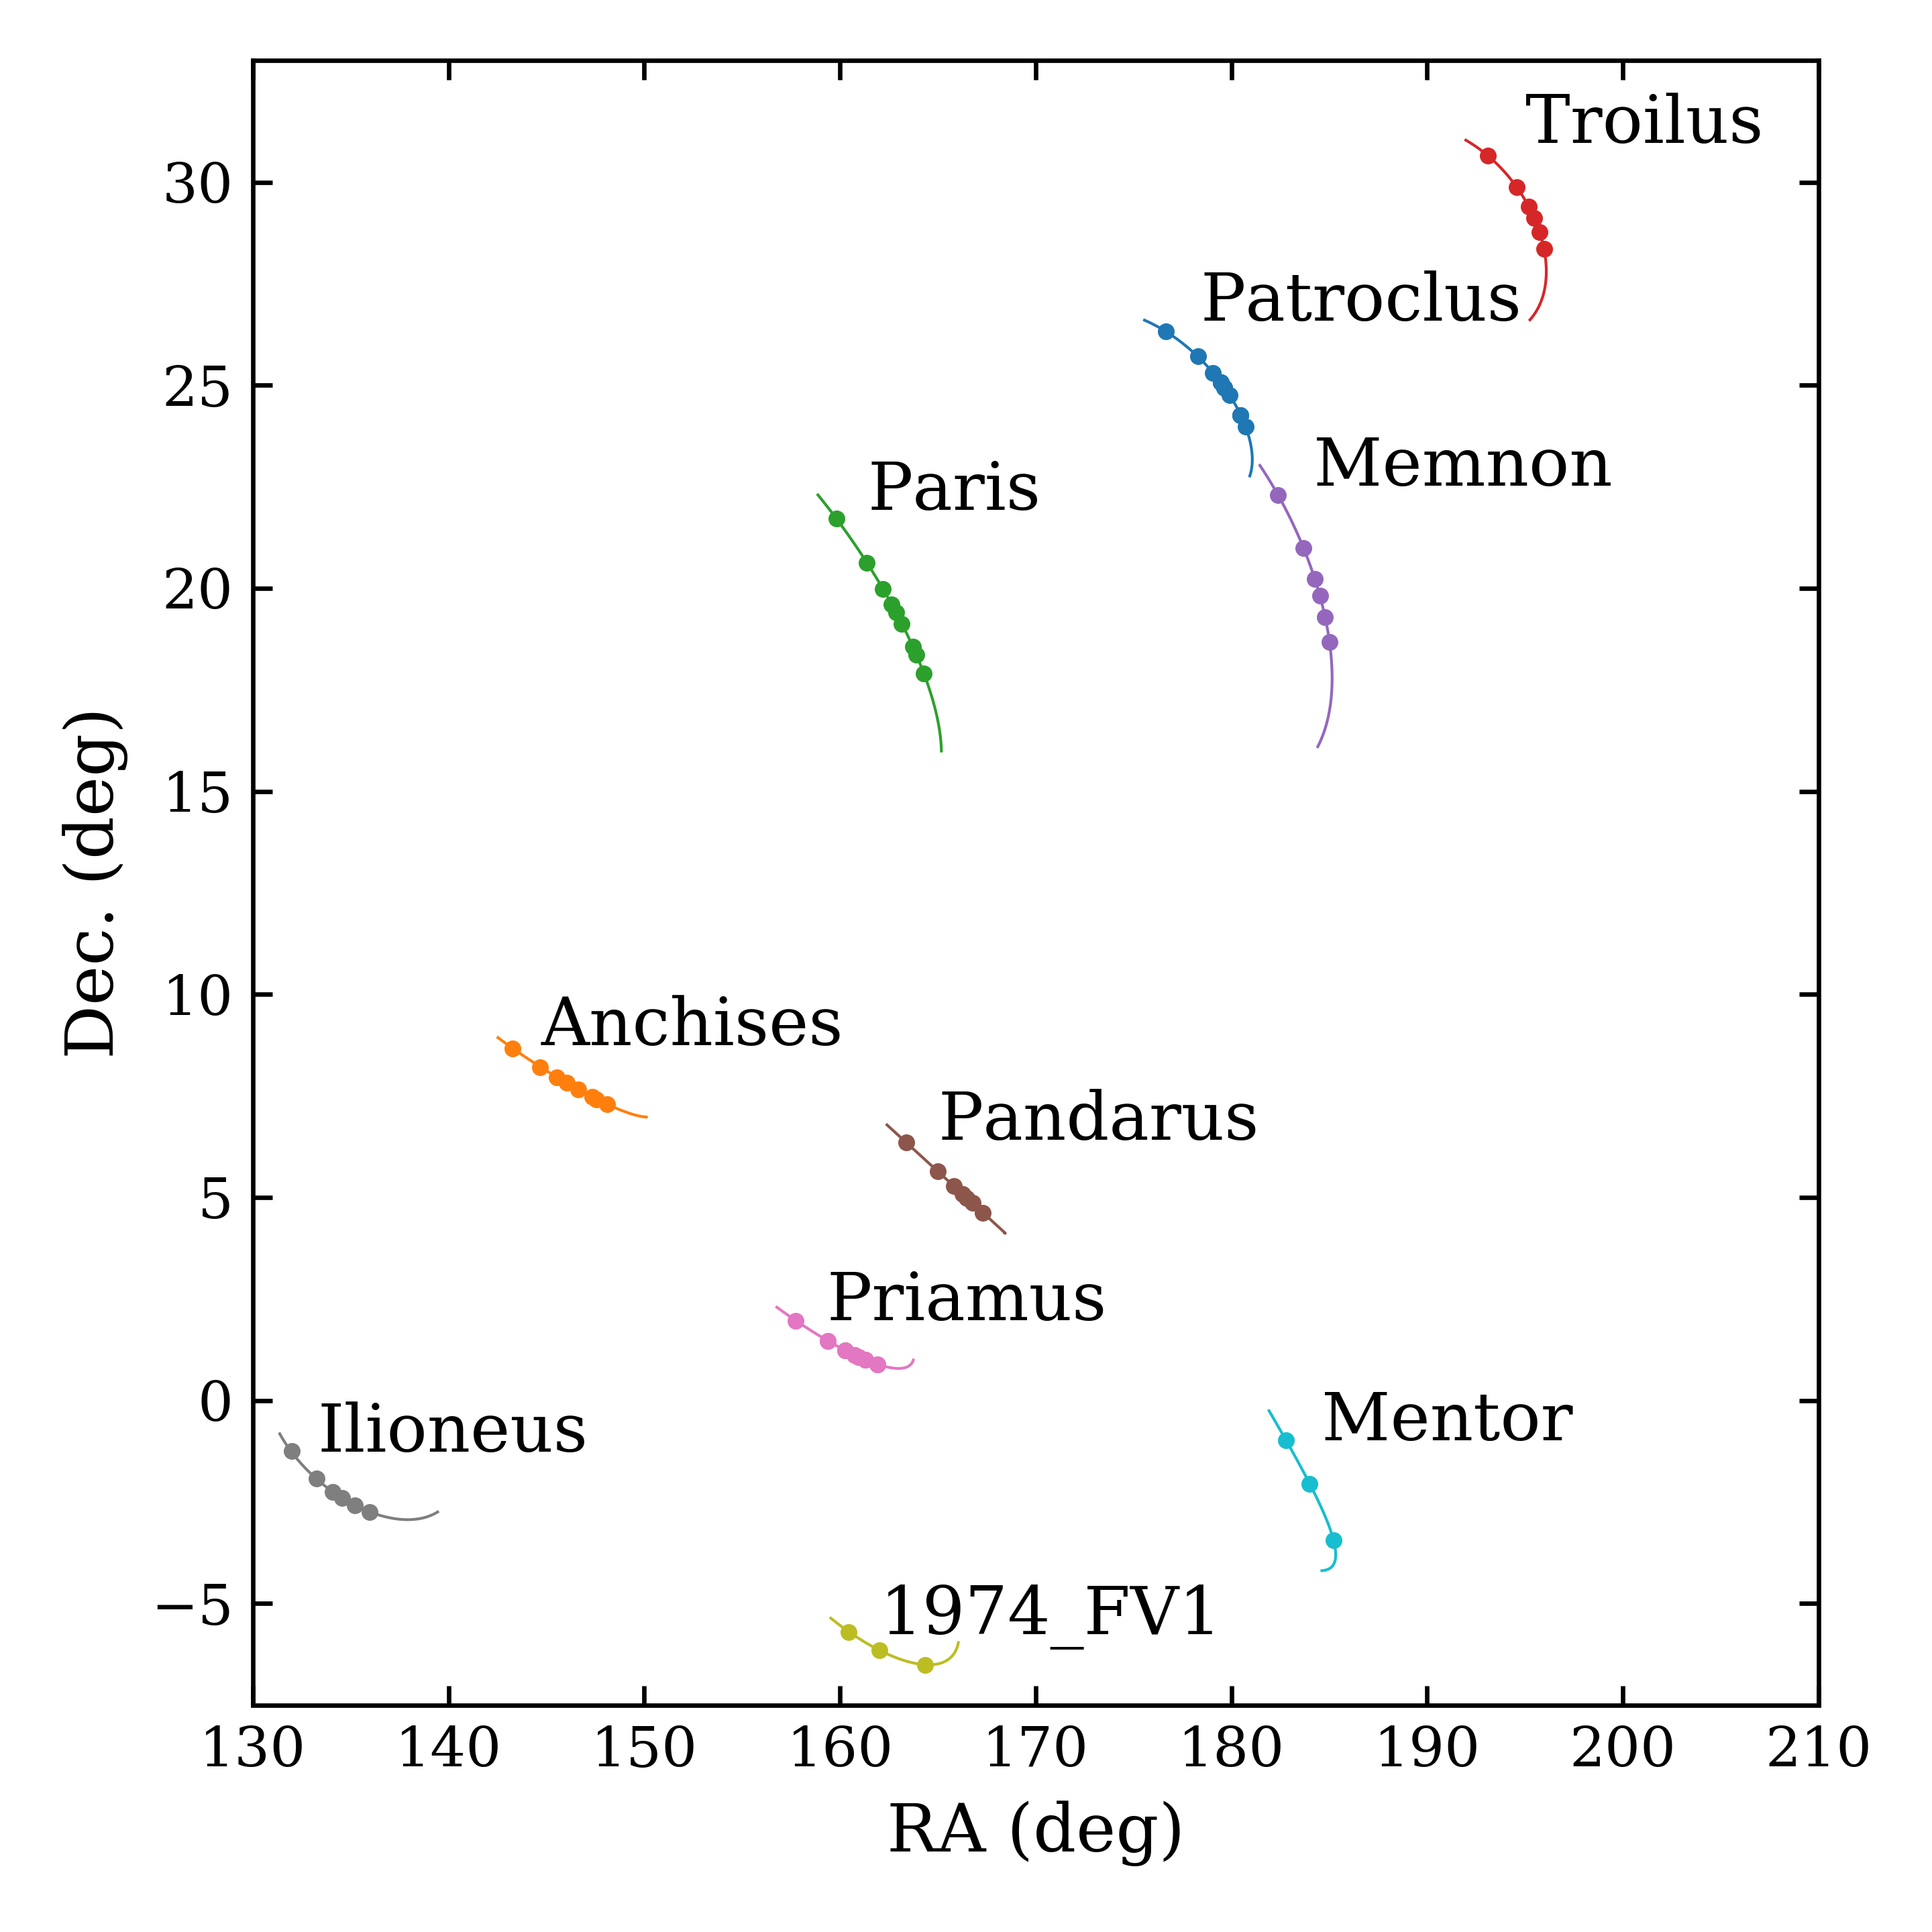
\includegraphics[width=0.5\textwidth]{20180402_115205_OBSERVATIONS_MAP}
\caption{Right-Ascensions and Declinations of asteroids acquired during our observations. Solid lines represent the expected movement of the asteroids during the 7 week observing period. The orbital parameters used were obtained from the IAU Minor Planet Centre.\scite{IAUMinorPlanet}}
\label{fig: observations}
\end{figure}

\begin{figure}[h!]
\centering
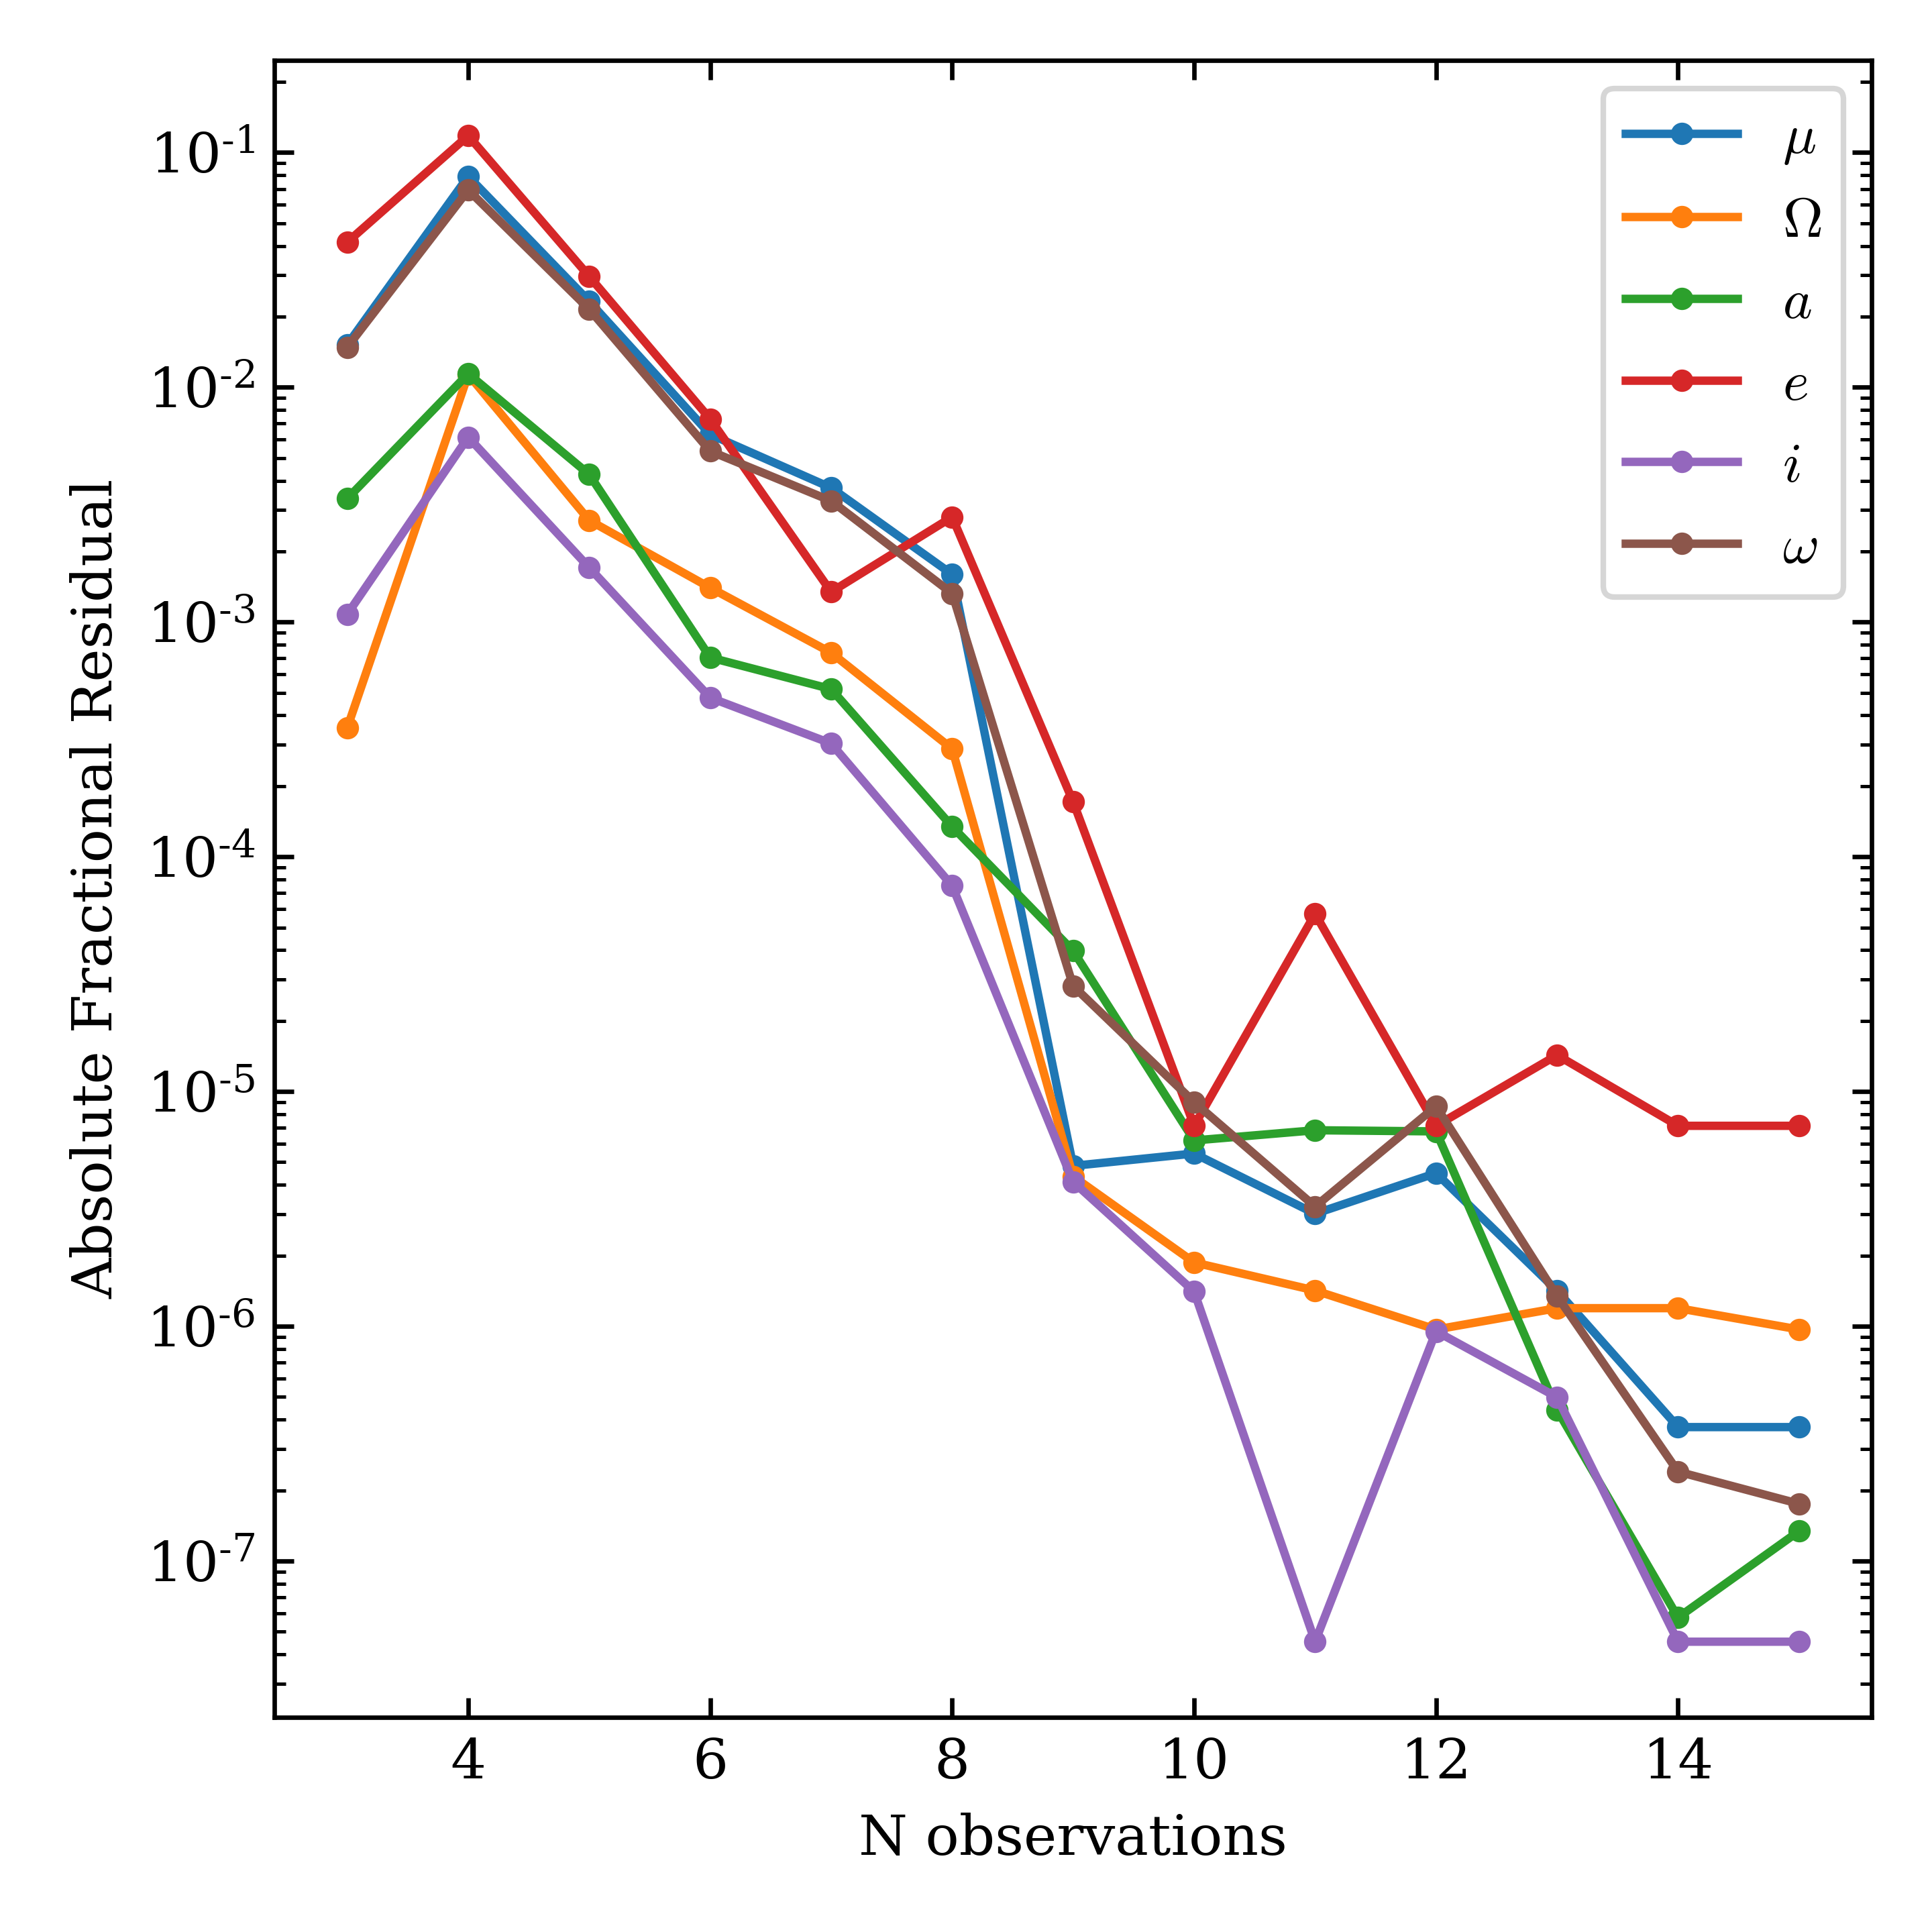
\includegraphics[width=0.5\textwidth]{20180402_155517_PAT_LIT_CONVERGENCE}
\caption{The absolute fractional residual between our calculated orbital parameters and the literature as the number of observations increases for Patroclus.}
\label{fig: pat convergence}
\end{figure}

\begin{figure}[h!]
\centering
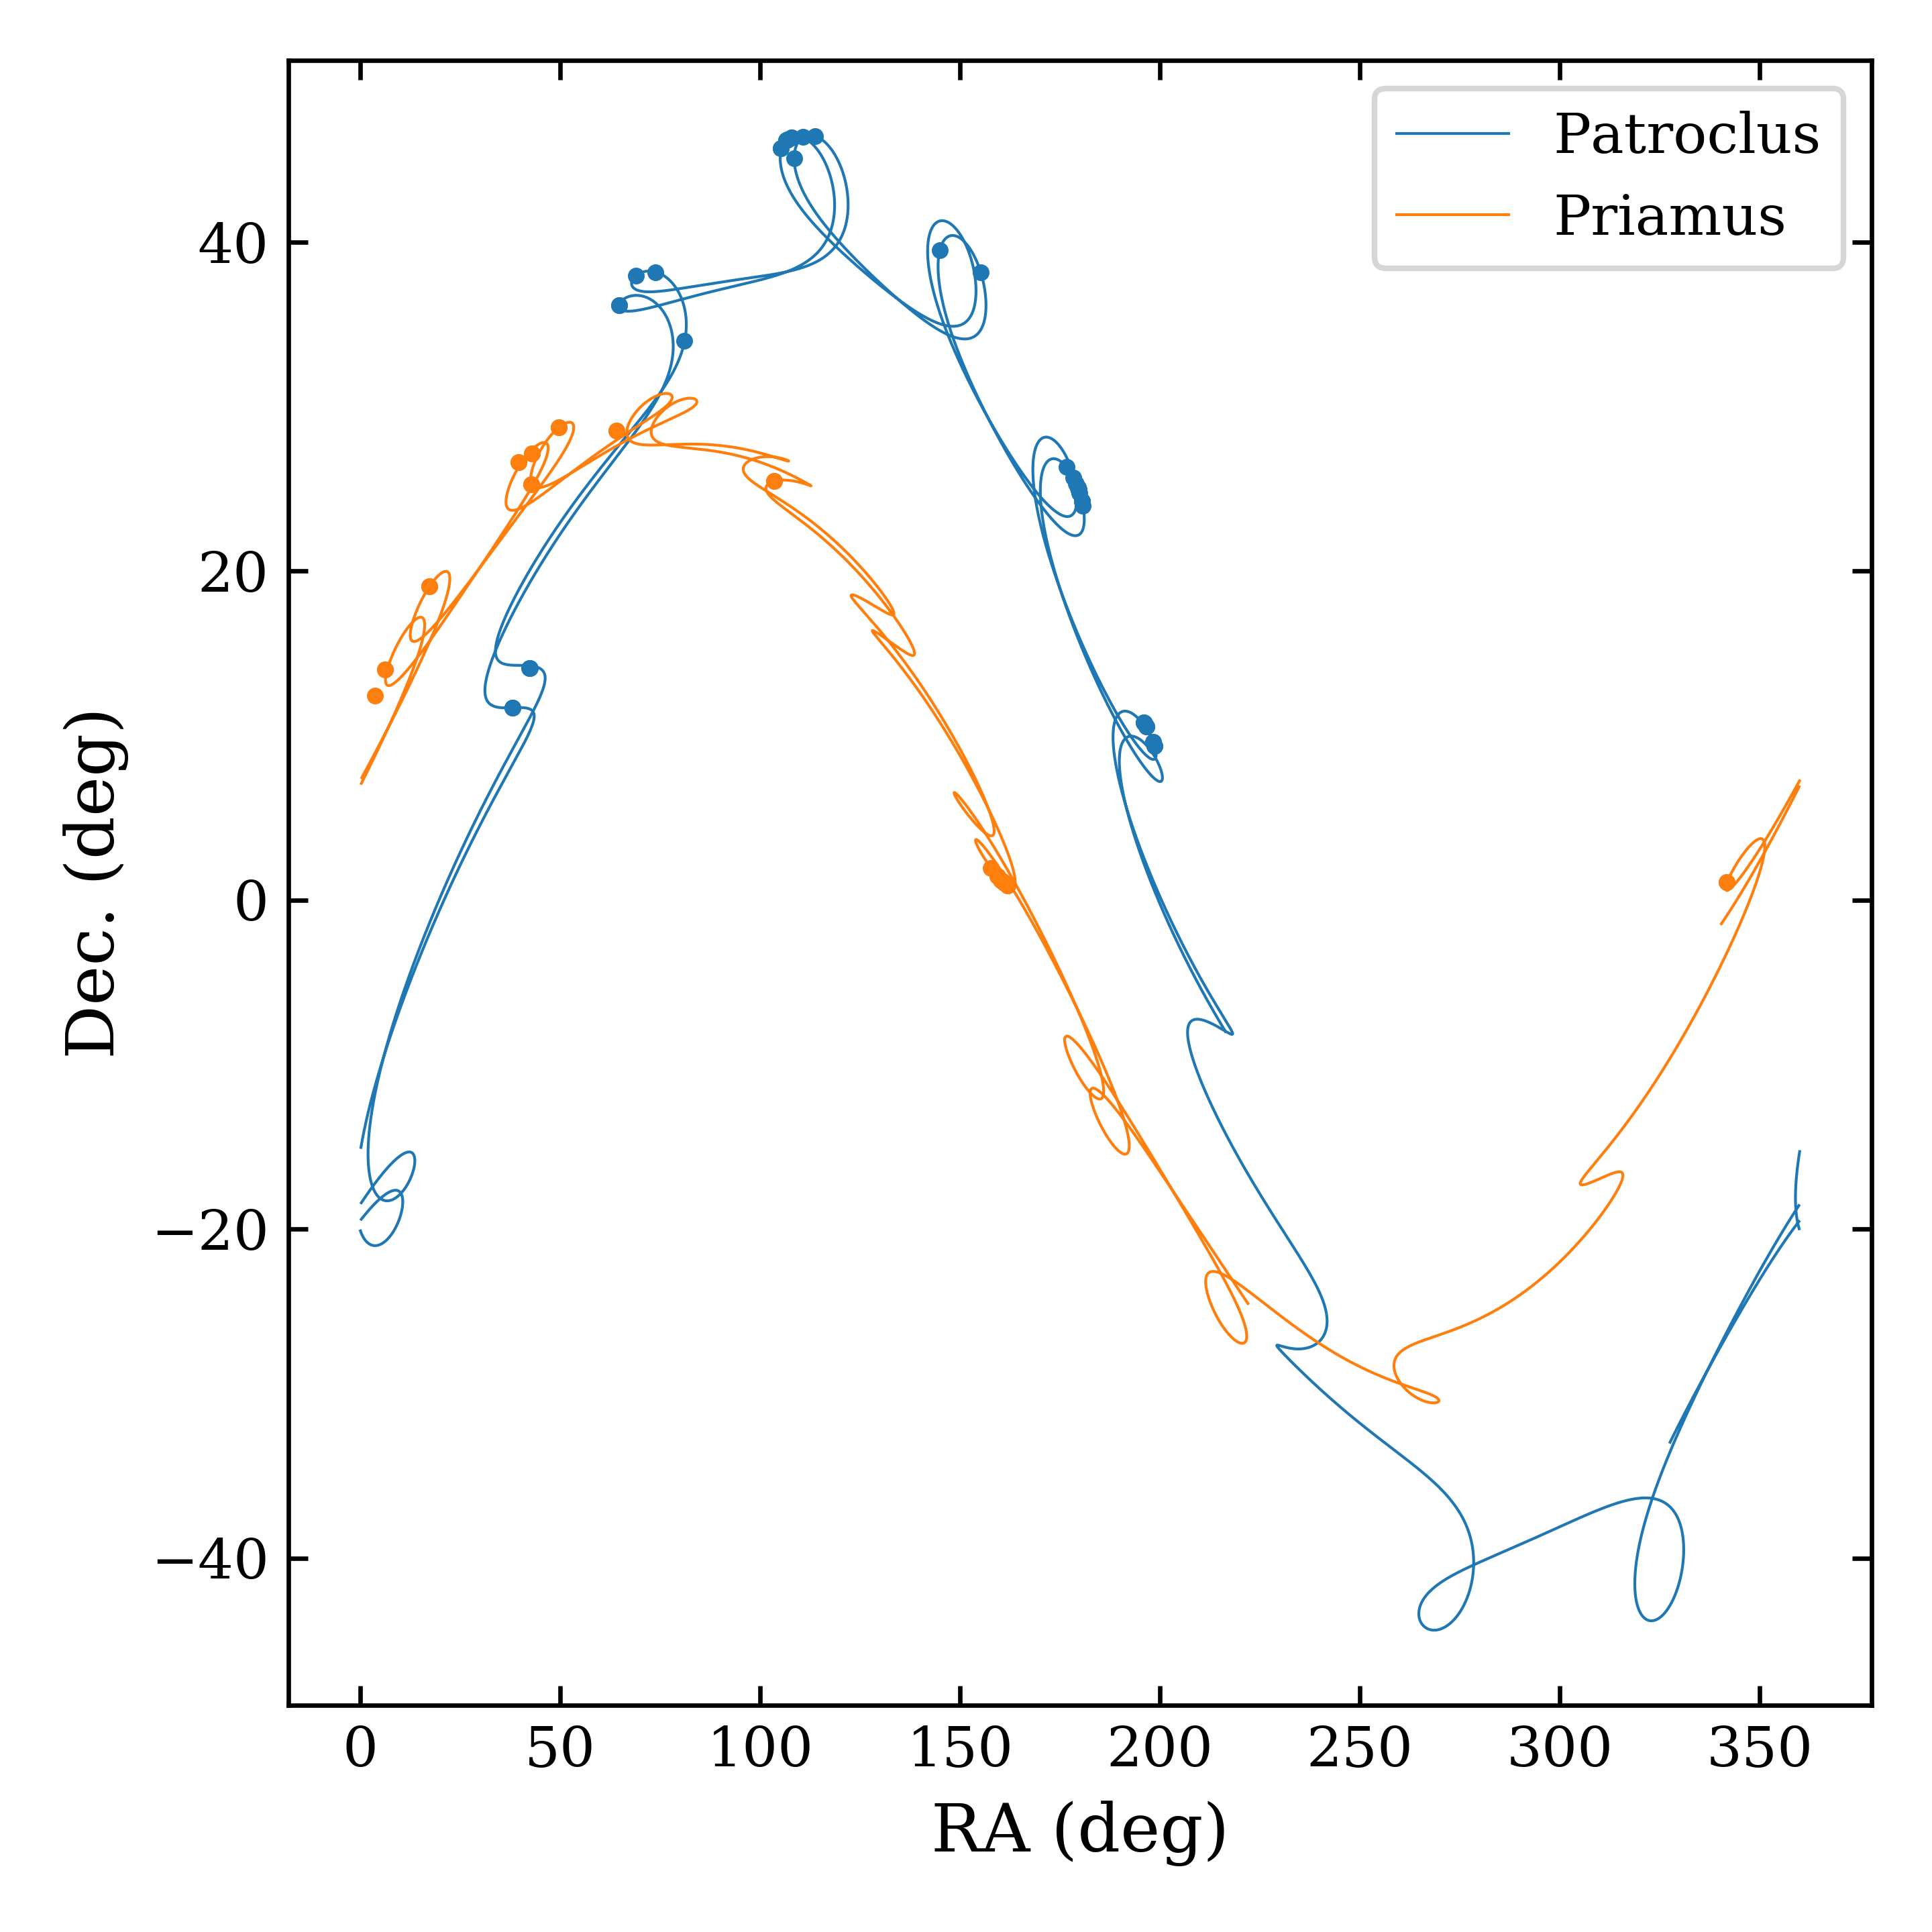
\includegraphics[width=0.5\textwidth]{20180402_171730_OBSERVATIONS_MAP}
\caption{The points represent the observations used to calculate their orbital parameters in Table \ref{tab: orbital parameters2}. The line represents its literature orbital path from the 1st January 2000 to the 1st January 2020. There are two distinct lines for each asteroid as the orbital period is ${\sim}12$ years and so each asteroid will complete ${\sim}1.7$ orbits.}
\label{fig: observations2}
\end{figure}

The Find\_Orb software was used to fit orbits to eight of our ten asteroids. 1974 FV1 and Mentor could not be fitted to orbits as only $3$ observations for each were attained. The jackknifing technique used to obtain errors on the orbital parameters requires at least 4 observations. The orbital parameters are given in Table \ref{tab: orbital parameters}.

These results demonstrate that the method used in this investigation is suitable for acquiring orbital parameters, as all parameters for 3 asteroids were found to match within $1\sigma$ error of the literature, and a further 4 asteroid's parameters found to within $3\sigma$ error of the literature. Ilioneus was the only asteroid that did not fall in either of these two groups which is most likely due to a lack of observations, as it was only observed on 4 nights. Table \ref{tab: orbital parameters} shows smaller errors were achievable with more observations. This is supported by Fig. \ref{fig: pat convergence} that shows that as the number of observations used in the orbit solution is increased, the results better converge to the literature value.

Our own observations can also be combined with archival data for Patroclus and Priamus to improve the accuracy of the calculated orbital parameters. The archival observations used are displayed in Fig. \ref{fig: observations2} and the improved orbital parameters are displayed in Table \ref{tab: orbital parameters2}.

Both sets of orbital parameters for Patroclus (from Table \ref{tab: orbital parameters} and Table \ref{tab: orbital parameters2}) were used to calculate its predicted position for the date of 2nd March 2033, this being the planned date for \textit{Lucy} to flyby Patroclus. The results of the predicted position are given in Table \ref{tab: patroclus position xyz} with error ellipsoids for their positions given in Fig. \ref{fig: pat position ellipsoid}. The ellipsoids shown in Fig. \ref{fig: pat position ellipsoid} provide the $3\sigma$ uncertainty in the asteroids position.

\begin{figure}[t!]
\centering
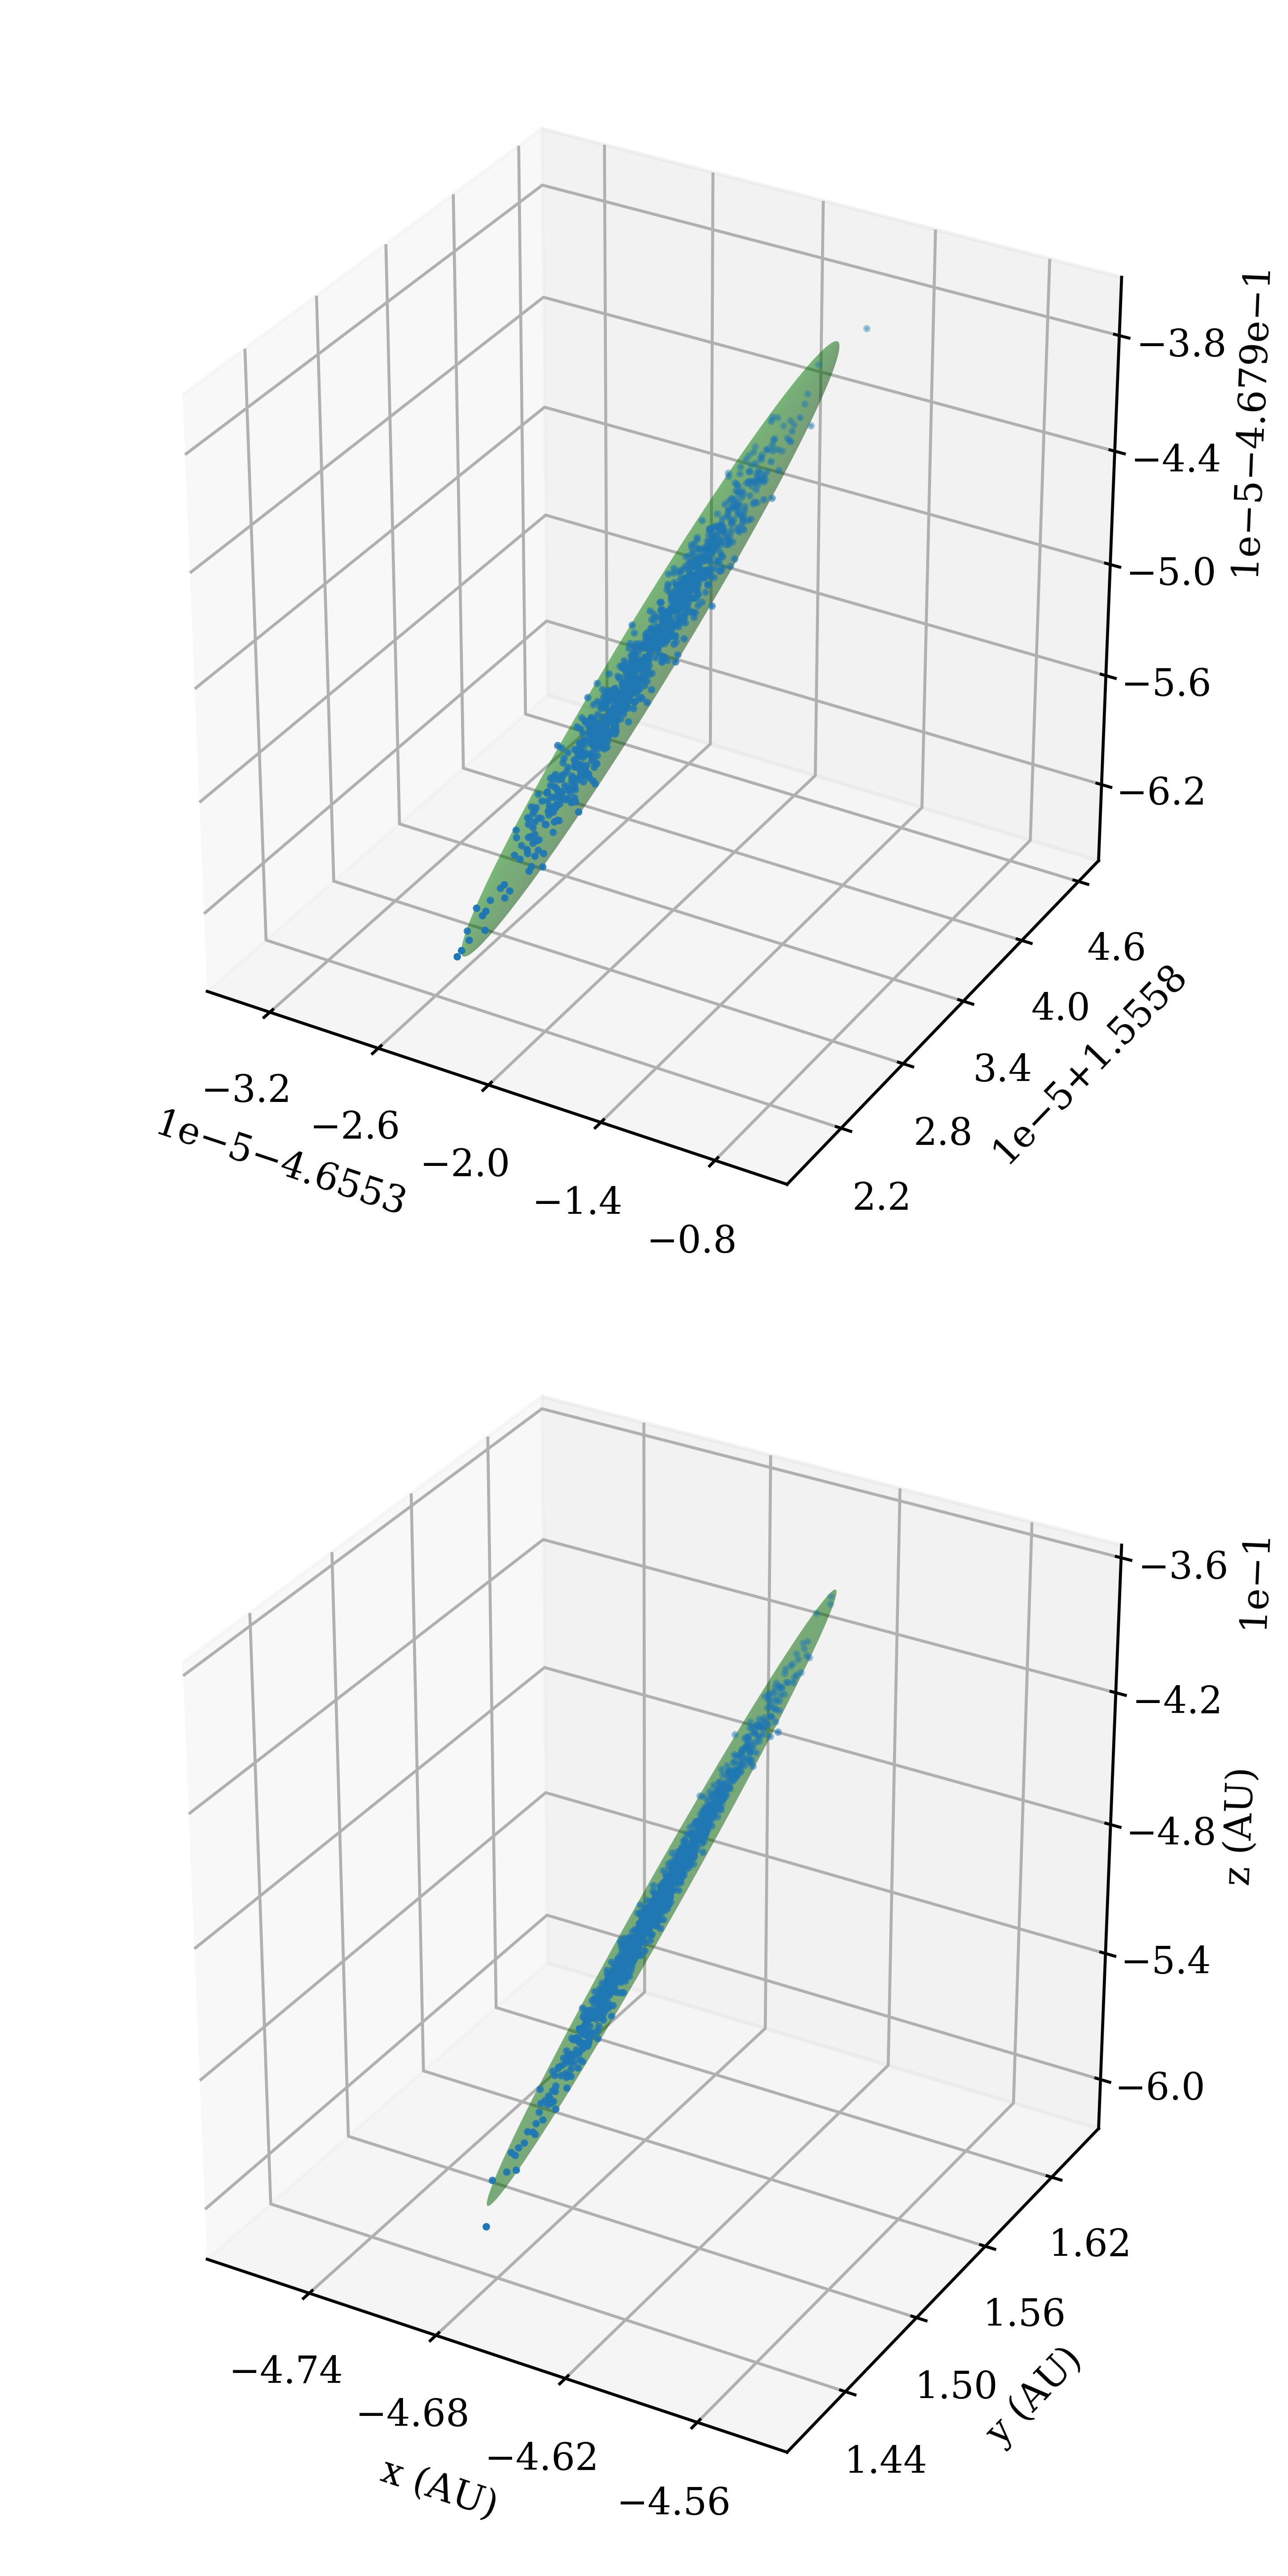
\includegraphics[width=0.45\textwidth]{20180411_125829_ERROR_ELLIPSOID_PAT}
\caption{The distribution of positions for Patroclus calculated from its orbital parameters including (top panel) and excluding (bottom panel) archival data. The error ellipsoid shown is at the $3\sigma$ confidence level.}
\label{fig: pat position ellipsoid}
\end{figure}

\begin{table}[ht!]
\centering
\begin{tabularx}{0.5\textwidth}{ Y Y Y Y }
\hhline{====}
& $x$ (AU) & $y$ (AU) & $z$ (AU) \\[3pt] \hline
Excluding archival data & $-4.655 \pm 0.006$ & $1.53 \pm 0.04$ & $-0.49 \pm 0.03$ \\[3pt]

Including archival data & $-4.6553203 \pm 0.0000009$ & $1.555832 \pm 0.000004$ & $-0.467951 \pm 0.000003$ \\[3pt] 

Literature & $-4.6553217$ & $1.555834$ & $-0.467952$\\[3pt] \hline

\end{tabularx}
\caption{The position of Patroclus on 2nd March 2033, the date of the \textit{Lucy} mission rendezvous. The uncertainties given are for a $1\sigma$ confidence region. The literature values given were calculated using the orbital parameters from JPL HORIZONS.}
\label{tab: patroclus position xyz}
\end{table} 

\begin{table}[ht]
\centering
\begin{tabularx}{0.5\textwidth}{ Y Y Y Y}
\hhline{====}
& Upper bound, $\Delta v_{T,u}$ (\si{\kilo\metre\per\second}) & Lower bound, $\Delta v_{T,l}$ (\si{\kilo\metre\per\second}) & $\frac{2( \Delta v_{T,u}-\Delta v_{T,l} )}{\Delta v_{T,u}+\Delta v_{T,l}}$ \\[3pt] \hline
Excluding archival data & $14.243$ & $14.236$ & $4.9 \times 10^{-4}$ \\[3pt]

Including archival data & $14.243685$ & $14.243684$ & $7.0 \times 10^{-8}$ \\[3pt] \hline

\end{tabularx}
\caption{The upper and lower bounds on $\Delta v_T$ for a Hohmann transfer to the positions in Table \ref{tab: patroclus position xyz} based on their errors. The fractional difference in the bounds is also displayed.}
\label{tab: upper lower bounds dv}
\end{table} 

These calculated positions can be used to place an upper and lower bound on the $\Delta v_{T}$ requirement for a Hohmann transfer in the plane of the orbit of the asteroid. These upper and lower bounds are given in Table \ref{tab: upper lower bounds dv}. The inclusion of archival data can significantly improve the range of the bounds, the fractional difference decreasing by four orders of magnitude from $4.9 \times 10^{-4}$ to $7.0 \times 10^{-8}$.

\begin{table*}[t]
\centering
\begin{tabularx}{\textwidth}{ Y Y Y Y Y Y Y Y Y }
\hhline{=========}

Asteroid &  & Mean Anomaly, $M$ ($\degree$) & Argument of Perihelion, $\omega$ ($\degree$) & Longitude of Ascending Node, $\Omega$ ($\degree$) & Semi-major axis, $a$ (AU) & Eccentricity, $e$ & Inclination, $i$ ($\degree$) & Number of Observations \\[3pt] \hline

\multirow{2}{*}{Anchises} & Observed & $294 \pm 2$ & $39 \pm 2$ & $284.2 \pm 0.2$ & $5.29 \pm 0.02$ & $0.147 \pm 0.006$ & $6.96 \pm 0.03$ & $7$ \\[3pt]
& Literature & $294$ & $41$ & $283.9$ & $5.31$ & $0.139$ & $6.91$ & \\[3pt] \hline

\multirow{2}{*}{Ilioneus} & Observed & $221 \pm 5$ & $220 \pm 10$ & $242.0 \pm 0.2$ & $5.6 \pm 0.1$ & $0.13 \pm 0.03$ & $15.48 \pm 0.08$ &  $4$ \\[3pt]
& Literature & $320$ & $112$ & $242.5$ & $5.23$ & $0.01$ & $15.7$ & \\[3pt] \hline

\multirow{2}{*}{Memnon} & Observed & $334 \pm 2$ & $277 \pm 2$ & $133.94 \pm 0.07$ & $5.239 \pm 0.002$ & $0.052 \pm 0.001$ & $27.20 \pm 0.04$ & $5$ \\[3pt]
& Literature & $336$ & $275$ & $133.98$ & $5.236$ & $0.051$ & $27.22$ & \\[3pt] \hline

\multirow{2}{*}{Pandarus} & Observed & $92 \pm 1$ & $41 \pm 1$ & $179.78 \pm 0.01$ & $5.182 \pm 0.002$ & $0.068 \pm 0.001$ & $1.856 \pm 0.002$ & $7$ \\[3pt]
& Literature & $92$ & $40$ & $179.79$ & $5.183$ & $0.068$ & $1.854$ & \\[3pt] \hline

\multirow{2}{*}{Paris} & Observed & $65.40 \pm 0.07$ & $150.61 \pm 0.04$ & $135.909 \pm 0.005$ & $5.2221 \pm 0.0001$ & $0.1270 \pm 0.0003$ & $27.852 \pm 0.006$ & $9$ \\[3pt]
& Literature & $65.61$ & $150.49$ & $135.918$ & $5.2222$ & $0.1278$ & $27.863$ & \\[3pt] \hline


\multirow{2}{*}{Patroclus} & Observed & $324.8 \pm 0.4$ & $308.2 \pm 0.3$ & $44.38 \pm 0.01$ & $5.220 \pm 0.001$ & $0.1398 \pm 0.0003$ & $22.049 \pm 0.002$ & $9$ \\[3pt]
& Literature & $325.2$ & $307.9$ & $44.37$ & $5.218$ & $0.1400$ & $22.053$ & \\[3pt] \hline

\multirow{2}{*}{Priamus} & Observed & $44.9 \pm 0.2$ & $335.1 \pm 0.1$ & $301.60 \pm 0.05$ & $5.173 \pm 0.002$ & $0.123 \pm 0.002$ & $8.912 \pm 0.009$ & $7$ \\[3pt]
& Literature & $44.8$ & $335.2$ & $301.64$ & $5.172$ & $0.124$ & $8.919$ & \\[3pt] \hline

\multirow{2}{*}{Troilus} & Observed & $247 \pm 2$ & $295 \pm 2$ & $48.56 \pm 0.03$ & $5.241 \pm 0.003$ & $0.0912 \pm 0.0005$ & $33.56 \pm 0.01$ & $6$ \\[3pt]
& Literature & $247$ & $295$ & $48.56$ & $5.240$ & $0.0911$ & $33.56$ & \\[3pt] \hline

\end{tabularx}
\caption{The calculated orbital parameters for 8 of our observed asteroids. The number of observations used to calculate the parameters is also given in the right-most column. The literature values were taken from JPL HORIZONS.\scite{HORIZONSSystem} The epochs of the literature and observed results were the same.}
\label{tab: orbital parameters}
\end{table*}

\begin{table*}[t]
\centering
\begin{tabularx}{\textwidth}{ Y Y Y Y Y Y Y Y Y }
\hhline{=========}

Asteroid &  & Mean Anomaly, $M$ ($\degree$) & Argument of Perihelion, $\omega$ ($\degree$) & Longitude of Ascending Node, $\Omega$ ($\degree$) & Semi-major axis, $a$ (AU) & Eccentricity, $e$ & Inclination, $i$ ($\degree$) & Number of Observations \\[3pt] \hline

\multirow{2}{*}{Patroclus} & Observed & $325.19538 \pm 0.00004$ & $307.85954 \pm 0.00003$ & $44.365937 \pm 0.000009$ & $5.2184995 \pm 0.0000001$ & $0.1399506 \pm 0.0000002$ & $22.052693 \pm 0.000005$ & $17$ \\[3pt]
& Literature & $325.19545$ & $307.85953$ & $44.365963$ & $5.2184997$ & $0.1399500$ & $22.052699$ & \\[3pt] \hline

\multirow{2}{*}{Priamus} & Observed & $44.7601 \pm 0.0002$ & $335.2247 \pm 0.0002$ & $301.63926 \pm 0.00008$ & $5.171862 \pm 0.000004$ & $0.1237472 \pm 0.0000009$ & $8.91919 \pm 0.00001$ & $17$ \\[3pt]
& Literature & $44.7607$ & $335.2235$ & $301.63945$ & $5.171847$ & $0.1237506$ & $8.91919$ & \\[3pt] \hline

\end{tabularx}
\caption{The calculated orbital parameters for 2 of our observed asteroids including the archival data. The number of observations used to calculate the parameters is also given in the right-most column.}
\label{tab: orbital parameters2}
\end{table*} 

\section{Discussion}

A preliminary investigation was performed to determine the accuracies of various star catalogues. For UCAC2, this found a systematic error of $0.2\pm0.1$ arcsecs in Dec. compared to the JPL HORZONS ephemeris. Initially, this was the star catalogue being used in our images, however, based on this result we took the decision to use astrometry based on the UCAC4 star catalogue as this was accurate to JPL HORIZONS within error. The decision to not use GAIA was based on that catalogue not having a full release published as yet. 

Our initial sample choice of asteroids provided good observations, with two asteroids, 1974 FV1 and Mentor, not producing enough observations to perform orbit determination. The low height of these asteroids in the sky resulted in observations not being possible on some nights where the rest of our asteroid sample was visible. Orbit determination was then run using the Find\_Orb software with all parameters for 3 asteroids within $1\sigma$ errors of the literature and all parameters for a further 4 asteroids within $3\sigma$ errors of the literature. The literature values were taken from JPL HORIZONS. The primary reason that only 3 asteroids were within $1\sigma$ errors is that our observations only ranged from the 24th January to the 10th March, a span of 45 days. As the approximate time period of a circular Trojan orbit is 12 years (4380 days), using our own observations we only covered an arc length of ${\sim}1\%$ of its total orbit which produces more inaccurate results with larger errors compared to a longer arc length.

It is shown trivially in Figures \ref{fig: JPL-find orb convergence} and \ref{fig: JPL-find orb convergence 18mth} that, generally, as the number of observations increases the orbital parameters better converge to the literature values. Fig. \ref{fig: JPL-find orb convergence 18mth} shows that increasing the time step between observations can produce more accurate results. This supports the notion that more accurate results can be achieved by maximising the observed arc length of its orbit.

We sourced archival data for Patroclus and Priamus to supplement our own observations, the orbital parameters were then recalculated. Using this archival data, the arc length of observations was significantly increased: for Patroclus, the earliest data obtained was from October 2001 and so we had sufficient data to cover ${\sim}1.4$ orbits; for Priamus, data was obtained from October 2011 and so we had archival data covering ${\sim}50\%$ of its total orbit.

These greater arc lengths allowed a solution with a far greater confidence to be calculated from our jackknifing method. The mean fractional uncertainty in our orbital parameters for Patroclus using only our own observations is $8.1 \times 10^{-4}$. This reduces by 3 orders of magnitude to $3.5 \times 10^{-7}$ when the archival data is included in the computation of the orbital parameters. We find similar improvements for Priamus which has a mean fractional uncertainty of $3.8 \times 10^{-3}$ using our own observations which reduces to $2.4 \times 10^{-6}$ including archival data. These results highlight the importance of supplementing our own observations with archival data allowing our $1\sigma$ confidence regions to be significantly reduced.  This is important to the aim of this investigation as these errors are propagated through to the calculation of Patroclus' position for the \textit{Lucy} rendezvous.

The orbital parameters calculated using archival data have significantly smaller error bars associated with them than compared to those calculated using only our own observations. Only 2 parameters are within $1\sigma$ error bars of the literature, however, if the error bars are extended to $3\sigma$, a further 7 are in agreement. The small differences between our values and the literature may not be due to errors in our method. These asteroids have osculating orbital parameters, meaning that they change over time. The JPL HORIZONS orbital parameters for Patroclus were calculated on 21st June 2017, whereas our orbital parameters use an epoch of osculation based on the mean date of our observations. As these parameters change over time, significant differences in epochs such as this are likely to be the cause of our results not aligning exactly with the literature.

Using our calculated orbital parameters for the prediction of Patroclus' position, we calculated the $1\sigma$ error ellipsoid based on the distribution of possible positions. The error ellipsoid has semi-major axis lengths equal to the eigenvalues of the covariance matrix of the position distribution. The volume of the $1\sigma$ ellipsoid calculated solely from our own observations is $1.7 \times 10^{-7}$ \si{AU^{3}}, whereas the volume of the ellipsoid found using orbital parameters including the archival data is $3.6 \times 10^{-18}$ \si{AU\cubed}. This is a significant improvement in confidence region with the volume decreasing by a factor of ${\sim}10^{11}$. 

This could make a highly significant difference to a NASA mission such as \textit{Lucy}, which has very limited constraints on resources such as fuel. To investigate the effect of this on the fuel requirements, the maximum radii from the error ellipsoids including and excluding archival data were used to find $\Delta v$ requirements of a Hohmann transfer. The calculated bounds on the $\Delta v_{T}$ requirements are given in Table \ref{tab: upper lower bounds dv}. These show that the difference in the bounds on the $\Delta v_{T}$ requirement can be significantly reduced if using a position of Patroclus with smaller error bars with the uncertainty in the $\Delta v_{T}$ requirement being reduced from $4.9 \times 10^{-4}$ to $7.0 \times 10^{-8}$ with the inclusion of the archival data. 

This reduction in the uncertainty of the $\Delta v_{T}$ requirement would be beneficial for the \Lucy mission as a high level of accuracy is required when performing orbital manoeuvrers and performing a flyby with the lowest possible separation with Patroclus. Highly accurate positions are required for rendezvous manoeuvres with minor planets to achieve an optimal flyby. However, this reduction in $\Delta v_{T}$ uncertainty would not be significantly beneficial in reducing the mass of the \Lucy mission as a fractional uncertainty of $4.9 \times 10^{-4}$ equates to $\Delta v \approx 7$ \si{\metre\per\second}, an amount largely negligible when considering $\Delta v_{T} \approx 14$ \si{\km\per\s} for the complete Hohmann transfer and hence the mass of fuel this would equate to would also be negligible.

\section{Conclusions}

Our investigation aimed to accurately determine the position of Patroclus for the \Lucy mission flyby. We did this by initially selecting 10 asteroids to study. Observations of these were taken using the Far-East 16, DRACO2 and Pt5m telescopes in the clear band over a period of 7 weeks. Before positional measurements could be taken from our images, the varying star catalogues were investigated.

The UCAC2, UCAC4 and GAIA star catalogues were compared to investigate their deviations from the JPL HORIZONS ephemeris calculator. UCAC4 and Gaia were found to be in agreement with JPL HORIZONS within error; however, UCAC2 was found to have a deviation from JPL HORIZONS of $0.2 \pm 0.1$ in declination. This was not surprising from an older star catalogue. Using these results, the UCAC4 catalogue was selected for use in this investigation.

Once the positions of our asteroids in terms of RA and Dec. were measured from our images, we used an implementation of the Gauss method to determine their orbital parameters. This implementation was verified and found to converge to the orbital parameters given by JPL HORIZONS. The orbital parameters were determined for $80\%$ of our initial asteroid sample; however, orbital parameters could not be determined for 1974 FV1 and Mentor as an insufficient number of observations were taken. Archival data was obtained for Patroclus and Priamus and supplemented with our own observations to determine improved orbital parameters for these asteroids.

All orbital parameters calculated using solely our own observations for 7 of our asteroids were found to be consistent with the literature within $3\sigma$ error bars. The main cause of inaccuracies is most likely the short arc of observation we had of our asteroids; our observations only covered ${\sim}1\%$ of the asteroid's full orbit. With the improved orbital parameters for Patroclus and Priamus, 9 of the 12 orbital parameters are in agreement with JPL HORIZONS. Inaccuracies in this case were most likely due to a difference in the epoch of osculation for our parameters, with our epoch being taken as the average day of observation. This differed to JPL HORIZONS which depended on when the calculation was performed. In the case of Patroclus, this was 21st June 2017.

We then used the orbital parameters for Patroclus to calculate its predicted position for the \Lucy mission rendezvous. The positions using orbital parameters including and excluding archival data were calculated. The confidence in the position including archival data was significantly higher than the position calculated excluding the archival data, the volume of the $1\sigma$ error ellipsoid reducing by a factor of ${\sim}10^{11}$.

An upper and lower bound of $\Delta v$ requirement for a Hohmann transfer was then calculated. The fractional uncertainty in the $\Delta v$ requirement could be reduced from $4.9 \times 10^{-4}$ to $7.0 \times 10^{-8}$. This is significant for performing an accurate orbital transfer as high level of accuracy is required when performing manoeuvres. When considering fuel requirements for the Hohmann transfer, a fractional uncertainty of $4.9 \times 10^{-4}$ equates to $\Delta v \approx 7$ \si{\metre\per\second}. This is negligible compared to the $\Delta v \approx 14$ \si{\kilo\metre\per\second} of the complete Hohmann transfer.
 
%Words \cite{MorbidelliChaoticcaptureJupiter2005a}

\vspace{1ex}
%\begin{acknowledgments}
%(OPTIONAL) The author would like to thank...
%
%\end{acknowledgments}
%
%
\normalem
\bibliographystyle{ieeetr} %UNCOMMENT THIS FOR BIB
\bibliography{Trojans} %UNCOMMENT THIS FOR BIB

\clearpage
\appendix

\section{Observing Log}

\begin{table}[h]
\centering
\begin{tabularx}{0.5\textwidth}{ Z Z Z Y }
\hline
\hline

Date (2018) & Telescope & Conditions & Objects Observed \\ \hline 
24th January & Far-East 16 & Cloudy & Anchises, Paris, Patroclus \\ \hline

29th January & Far-East 16 & Cloudy/Clear & Anchises, Paris, Patroclus \\ \hline

31st January & Far-East 16 & Cloudy/Clear & 1974 FV1, Anchises, Ilioneus, Memnon, Mentor, Pandarus, Paris, Patroclus, Priamus, Troilus \\ \hline

6th February & Far-East 16 & Cloudy/Clear & Anchises, Ilioneus, Memnon, Pandarus, Paris, Patroclus, Priamus, Troilus \\ \hline

9th February & DRACO2 & Clear & Pandarus, Paris, Patroclus, Priamus \\ \hline

11th February & DRACO2 & Clear & Anchises, Ilioneus, Memnon, Pandarus, Paris, Patroclus, Priamus, Troilus \\ \hline

15th February & Far-East 16 & Clear & Anchises, Ilioneus, Memnon, Pandarus, Paris, Patroclus, Priamus, Troilus \\ \hline

22nd February & Far-East 16 & Cloudy/Clear & 1974 FV1, Anchises, Ilioneus, Memnon, Mentor, Pandarus, Paris, Patroclus, Priamus, Troilus \\ \hline

7th March & Far-East 16 & Clear & 1974 FV1, Anchises, Ilioneus, Memnon, Mentor, Pandarus, Paris, Patroclus, Priamus, Troilus \\ \hline

10th March & Pt5m & Cloudy & Patroclus \\ \hline

\end{tabularx}
\caption{A record of the observations taken during the course of this investigation.}
\label{tab: observing log}
\end{table} 

\begin{table}[H]
\centering
\begin{tabularx}{0.5\textwidth}{ A Y }
\hline
\hline

Asteroid & Observations \\ \hline

Patroclus & 27th October 2001, 26th January 2003, 1st February 2004 5th February 2007, 17th October 2013, 24th September 2014, 13th January 2015, 13th March 2016, 12th January 2017 \\ \hline

Priamus & 15th October 2011, 9th October 2012, 29th October 2013, 23rd January 2014, 2nd February 2016 \\ \hline 

\end{tabularx}
\caption{A record of the archival observations used in this investigation.}
\label{tab: archival log}
\end{table} 


Table \ref{tab: observing log} gives a detailed observing log of all observations taken during the course of this investigation. Given in Table \ref{tab: archival log} is a record of all archival observations used in this investigation.

\section{Error Ellipses for Patroclus Position} \label{app: error ellipses}

The errors in the position of Patroclus were calculated using the covariance matrix of the distribution of positions. The covariance matrix, $\mathbf{C}$, for the positions is given below:
\begin{equation}
\mathbf{C} = 
\begin{bmatrix}
E_{xx} & E_{xy} & E_{xz} \\
E_{yx} & E_{yy} & E_{yz} \\
E_{zx} & E_{zy} & E_{zz} \\
\end{bmatrix},
\end{equation}
where $E_{ij} = E[(i - \mu_i)(j - \mu_j)],\ i,j = X,Y,Z$; $E$ is the expectation operator; $X,\ Y,\ Z$ are the corresponding set of Cartesian coordinates; $\mu_X,\ \mu_Y,\mu_Z$ are the mean of the corresponding Cartesian coordinate set.

The root of the diagonal elements of $\mathbf{C}$, $E_{xx},E_{yy},E_{zz}$, are used as the error in each Cartesian coordinate. Explicitly:
\begin{align}
\sigma_x &= \sqrt{E_{xx}}, \\
\sigma_y &= \sqrt{E_{yy}}, \\
\sigma_z &= \sqrt{E_{zz}},
\end{align}
where $\sigma_x,\sigma_y,\sigma_z$ is the error in the respective Cartesian coordinate and these are the errors used in Table \ref{tab: patroclus position xyz}.

The eigenvalues, $\lambda_1,\ \lambda_2,\ \lambda_3$; and eigenvectors, $\mathbf{v}_1,\ \mathbf{v}_2,\ \mathbf{v}_3$; of $\mathbf{C}$ can then be found to construct the error ellipsoid. The roots of the eigenvalues represent the semi-axis lengths of the ellipsoid. The ellipsoid is rotated so that each eigenvalue semi-axis length is aligned in the direction of its corresponding eigenvector.

\section{Computational Programs}

All code used to produce the results in this investigation is available here: \url{https://github.com/baldimort/Trojans-Lucy-Mission}.

\end{document}